% C2GES Information-format revision, 20 September 2026 (migrated from the Applied Sciences diagnostic submission).
% MDPI class: Definitions/mdpi.cls v6.5a (2026-09-11 official ACS template).
% All post-access evidence is labeled exploratory; the RSI 15-test comparison is
% held-out-for-this-revision, not unseen confirmatory. No human validation is claimed.
\documentclass[information,article,submit,moreauthors]{Definitions/mdpi}
\firstpage{1}
\makeatletter\setcounter{page}{\@firstpage}\makeatother
\pubvolume{1}\issuenum{1}\articlenumber{0}\pubyear{2026}\copyrightyear{2026}
\datereceived{}\daterevised{}\dateaccepted{}\datepublished{}
\newcommand{\cges}{C\textsuperscript{2}GES}
\setlength{\headheight}{20pt}
\AtBeginDocument{\pdfstringdefDisableCommands{\def\cges{C2GES}}}

\Title{C\texorpdfstring{\textsuperscript{2}}{2}GES: A Diagnostic Evaluation of Role-Conditioned Extractive Summarization for Long Power-System Technical Reports}
% ORCID: none declared for either author on 24 August 2026; per the MDPI template, ORCID commands are omitted.
\Author{Bijing Liu $^{1,2}$ and Yong Yang $^{1,2,}$*}
\AuthorNames{Bijing Liu and Yong Yang}
\address{$^{1}$ \quad NARI Group Corporation (State Grid Electric Power Research Institute), Nanjing 211106, China;\\
$^{2}$ \quad Beijing Kedong Electric Power Control System Co., Ltd., Beijing 100080, China}
\corres{Correspondence: yangyong1@sgepri.sgcc.com.cn}

\abstract{Role-conditioned extraction adds role evidence, a typed proxy graph, and a path-deletion term to lexical relevance; this diagnostic evaluation asks which layer carries measurable information for long power-system reports. \cges{} is a deterministic, source-linked selector with inspectable channels. The role layer carries measurable effects: on a seven-series pilot, role evidence raised ROUGE-L by 0.0186 at 260 words (interval [0.0078, 0.0320]), and its cues matched professionally annotated spans at precision 0.610 and 0.807 against base rates near 0.52, with recall near 6\%. The typed path layer is the layer that failed: Full-minus-no-path was -0.00799/-0.00718 in the pilot. On 15 North American Electric Reliability Corporation (NERC) reports, Full exceeded Semantic-MMR and TextRank at equal unit counts, the only corrected internal win, but produced 54--63\% longer outputs; the unrenormalized removal comparison is scale-coupled. A freeze-before-eval redesign scored 0.0652/0.1044 against 0.0654/0.1020 (held-out, not unseen). On a prospectively frozen external corpus of 19 reports it fell below no-path at 260 words after correction, while an untyped baseline exceeded it. Eight fictional fixtures are not real data. The evidence supports this component-level diagnosis, not superiority, proxy validity, or operational benefit.}
\keyword{extractive summarization; diagnostic evaluation; negative results; power-grid reports; length-controlled evaluation; reproducibility}
% Featured Application removed for the Information submission: mdpi.cls emits that
% block for any journal whenever the command is non-empty, but the section belongs
% to Applied Sciences and MDPI Information has no equivalent. Its content is covered
% by the abstract and the Introduction.

\begin{document}

\section{Introduction}

Power-system reliability and event-analysis reports often extend across hundreds of pages. Evidence about an initiating condition, a trigger, system propagation, consequences, and corrective action may appear in different sections and coexist with tables, standards language, recommendations, and appendices. Engineers reviewing such material need more than a list of individually prominent sentences. They need a compact route through structurally complementary passages and a reliable way to return to the source.

Extractive summarization is attractive in this setting because it preserves the wording and location of selected passages. Position, centroid-style lexical relevance, graph centrality, and semantic diversity provide useful ranking signals \cite{zhong2020extractive,bi2021aredsum,liu2021unsupervised,mihalcea2004textrank,reimers2019sentencebert}. These signals, however, do not necessarily distinguish the roles that passages play in an engineering account. A highly central passage may repeat background information, whereas a less central passage may contain the only mitigation or consequence needed to interpret an event.

Graph-based summarizers model relationships among sentences through learned graphs, hypergraphs, or structural filtering \cite{siragusa2022sentencegraph,onan2024mches,hark2025mis}. Power-domain language studies use entity--relation extraction and knowledge graphs to organize fault, alarm, and inspection evidence \cite{liu2022powerfault,ma2025alarm,zgg2026bridge}. \cges{} links these lines of work in an engineering-oriented formulation: candidate units receive transparent textual roles, compatible roles form typed paths, and path participation is combined with relevance, graph salience, position, and redundancy control. Each selected unit remains linked to its original report page.

The study uses complete public reliability, disturbance, event-analysis, recommendation, and assessment reports from the North American Electric Reliability Corporation (NERC). NERC guidance on the attributes of quality event-analysis reports provides the institutional context for this report family \cite{nerc2015qualityreport}. These reports contain event narratives and corrective lessons but are not utility work orders, inspection records, or field-maintenance narratives. The corpus is therefore treated as a maintenance-oriented technical-report proxy. Twelve reports support development, and 15 reports form the retained test set. All candidates are drawn from report pages outside the official Executive Summary, which is used only as the reference for automatic evaluation.

Beyond its summarization framing, the question this study turns on is an information one: does a typed structural representation supply discriminative information that lexical relevance and dense embedding similarity do not already carry, or does it merely re-encode what those signals already supply? The distinction has consequences beyond this corpus: if the typing is redundant, the graph machinery adds representational cost without adding extractable information, and a simpler untyped representation is the better instrument. This diagnostic study asks four bounded questions. \textit{RQ1} asks whether the apparent retained-test advantage persists after output length and report-series dependence are examined and whether the same ordering appears in a separately identified post-access pilot with matched 110- and 260-word budgets. \textit{RQ2} asks which role, reservation, graph, path, and redundancy components change performance or selection behavior in controlled exploratory variants. \textit{RQ3} asks what extraction defects and role disagreements are exposed by an explicitly non-human two-model audit, without treating machine agreement as construct validation. \textit{RQ4} asks whether a path channel redesigned under a freeze-before-evaluation protocol clears the no-path reference on held-out reports at those budgets, and what a synthetic stress set shows about software and endpoint alignment.

The paper makes three current contributions. First, it diagnoses which layer of the role-conditioned design carries measurable information: role evidence and role-group reservation show the largest component effects measured here, whereas the typed path-deletion layer does not improve the predefined endpoint and is detectably below no-path on a frozen external corpus at the larger budget. Second, it supplies the deterministic, source-linked selector and the evaluation boundary that make that diagnosis admissible, namely length-controlled budgets, series-level clustering, exact enumeration, and a freeze-before-evaluation revision. Third, it reports the resulting system comparison as budget- and corpus-dependent rather than uniform. The negative component result is: path deletion did not improve the predefined retained-test endpoint, was negative relative to no-path in the exploratory word-budget pilot, and typed edge information showed no stable exploratory advantage over an untyped graph. Taken together, these results do not establish that role typing contributes extractable information beyond the untyped graph; on the evidence collected, the simpler representation is the defensible default. Stronger confirmatory and semantic-validity claims are reserved for future independently collected evidence and are not contributions of this submission.

\section{Related Work}

\subsection{Extractive Technical-Document Summarization}

Extractive methods rank source sentences using position, document-centroid similarity, graph centrality, learned salience, or redundancy-aware relevance \cite{zhong2020extractive,bi2021aredsum,liu2021unsupervised}. Extractive summarization is itself an information-extraction process, and the question this study measures is which of those signals contribute independently to the measured endpoint. Lead and centroid methods remain useful controls, while TextRank and LexRank provide widely used graph-ranking references \cite{mihalcea2004textrank,erkan2004lexrank}. Dense sentence representations extend lexical matching and support semantic relevance--diversity selection \cite{reimers2019sentencebert}. History-conditioned selectors go further and make each choice with the partial extract in view: MemSum casts selection as a multi-step episodic Markov decision process, so redundancy is discounted by state rather than by a fixed penalty \cite{gu2022memsum}. The selector studied here keeps a fixed redundancy penalty (Equation~\eqref{eq:redundancy}) for determinism and auditability; calibrating or adapting that coefficient is deferred to the pre-frozen external protocol (Section~\ref{sec:future-validation}). Holding candidates, references, preprocessing, and extraction-unit budgets constant allows these ranking principles to be compared within one report corpus, although representation and tuning opportunities still differ.

PacSum augments thresholded sentence centrality with asymmetric weights for preceding and following positions \cite{zheng2019pacsum}. It is included as a modern unsupervised comparator because it combines semantic similarity, graph centrality, and position without supervised summary labels. The controlled implementation is explicitly named PacSum-MiniLM: it independently implements the published centrality equations while using the same fixed MiniLM representation and long-unit policy as Semantic-MMR in the exploratory pilot. It is therefore not presented as a byte-equivalent reproduction of the authors' task-fine-tuned BERT implementation. STAS ranks sentences from hierarchical Transformer attentions pretrained on unlabeled news documents \cite{xu2020stas}; Bi-GAE pretrains sentence--word bipartite embeddings for TextRank- or PacSum-style ranking \cite{mao2023bigae}. Neither method was scored on the retained 15-report NERC test, and neither is a substitute for the typed-path ablation reported here. Same-journal work reports graph-based extractive sentence scoring for large corpora \cite{verma2023graph} and full summarization evaluation campaigns on domain documents such as legal case law \cite{koniaris2023legal} and Urdu news \cite{azhar2025urdu}; those studies compare complete systems under their own corpora, lengths, and languages, which is the reason this study asks a prior and narrower question about how much of a structural advantage survives an information-matched component comparison.

Long technical documents add layout and discourse problems that are less prominent in short news articles. Bug-report summarization, for example, must distinguish problem statements, observed behavior, diagnostic discussion, and resolution-oriented passages \cite{koh2022bugreport}. Multi-document methods must likewise balance common content against source-specific evidence \cite{zhang2024tomds}. NERC reports combine long narrative sections with tables, standards language, recommendations, and appendices. This motivates a selector that considers both sentence relevance and the role of a passage in the report's engineering account. A same-journal evaluation of structured summarization against expert-curated properties pairs automatic semantic measures with a human assessment survey \cite{nechakhin2024orkg}; the present study follows that division of labour by reserving construct validity for the annotated study described in Section~\ref{sec:human-validation-protocol} instead of inferring it from reference overlap.

\subsection{Graphs, Semantic Ranking, and Causal Language}

Graph summarizers model relations among sentences, entities, topics, or discourse units \cite{wang2020heterogeneous,cui2020enhancing,jing2021multiplex}. Learned sentence graphs, contextual hypergraphs, independent-set filtering, and heterogeneous long-document graphs all extend isolated relevance scoring \cite{siragusa2022sentencegraph,onan2024mches,hark2025mis,bugueno2025graphlss}. GraphLSS learns heterogeneous lexical, structural, and semantic edges on long documents \cite{bugueno2025graphlss}; \cges{} instead uses deterministic role-typed proxies and does not train edge labels. StrucSum injects sentence-graph structure into prompts for zero-shot extractive summarization of long documents and reports that combining its structural prompting strategies does not clearly improve performance \cite{yuan2026strucsum}. That null concerns prompt-level combinations on general-domain corpora rather than typed against untyped edges on a domain report family, but it is a negative structural result in the same problem setting, and we record it as the closest published analogue of the component question asked here. \cges{} takes a complementary approach. It uses fixed lexical roles and deterministic typed-path enumeration so that the contribution of each score channel and selected sentence can be inspected.

The graph is rebuilt for each report and does not store a persistent asset ontology. Its node-deletion term measures how much qualified textual-path utility is lost when one sentence node is removed. This is a structural sensitivity feature, not an alternative physical event. Causal NLP distinguishes language association from intervention and counterfactual identification \cite{feder2022causal,du2022ecare}; accordingly, the present method is described as causal-chain-inspired only in the sense of its condition--event--impact--mitigation role progression. The remainder of the paper uses the more precise term \emph{path-deletion term}.

\subsection{Power-Grid Text Analytics}

Grid language technologies cover infrastructure analysis, digital twins, supervised entity--relation extraction, and persistent knowledge graphs \cite{xie2022massively,hamann2024foundation,madabhushi2023survey,srinivasan2023artificial,ranawaka2024leveraging,meng2023gridfield}. Power-fault, line-loss, and alarm-tracing graphs organize entities or events \cite{liu2022powerfault,li2024lineloss,ma2025alarm}. Maintenance-oriented retrieval and knowledge-graph studies use equipment or inspection records and sometimes include annotation or practitioner evaluation \cite{cao2024coalmaintenance,zgg2026bridge,dimaggio2025predictivemaintenance}. Relation-extraction methods similarly predict supervised entity--relation labels \cite{li2025moere,she2025clear}.

\cges{} addresses a different level of analysis: it ranks passages from a complete report while preserving source locations and encouraging complementary textual roles. Table~\ref{tab:related-comparison} positions this formulation against selected adjacent studies. The contribution evaluated here is the integration of deterministic role evidence, typed-path participation, source-linked extraction, and a strict component ablation. The study claims neither absolute priority over adjacent methods nor a performance benefit from the current path-deletion term.

\begin{table}[H]
\caption{Positioning against selected studies with related structural or power-domain objectives.}
\label{tab:related-comparison}\centering\scriptsize
\begin{tabularx}{\textwidth}{p{2.5cm}p{2.4cm}p{2.5cm}p{2.5cm}X}
\toprule
Study family & Primary object & Structural mechanism & Evaluation emphasis & Difference from this study\\
\midrule
Sentence Graph Attention / MCHES \cite{siragusa2022sentencegraph,onan2024mches} & General-domain documents & Learned sentence graph or contextual hypergraph & Summary metrics on benchmark corpora & Learned semantic representations; no NERC proxy or node-deletion ablation\\
Graph MIS + LLM \cite{hark2025mis} & DUC and CNN/DailyMail documents & Independent-set filtering and graph metrics & ROUGE and computational efficiency & Different graph objective, corpora, and generation components\\
Bug-report summarization \cite{koh2022bugreport} & Software issue reports & Learned sentence significance & Technical-artifact summary quality & Similar long technical discourse, but different roles, references, and domain\\
Power fault/alarm graphs \cite{liu2022powerfault,ma2025alarm} & Power-domain entities and events & Ontology/KG extraction and graph tracing & Entity, relation, or tracing performance & Structured knowledge construction rather than report-level extractive summarization\\
Maintenance KG and retrieval \cite{cao2024coalmaintenance,zgg2026bridge} & Equipment or inspection records & LLM retrieval or ontology-constrained extraction & Retrieval, annotation, manual audit, or practitioner utility & Title-concordant data and human assessment; no comparable extractive ablation\\
\cges{} & Selected NERC technical reports & Deterministic role graph and typed-path deletion & Executive-Summary overlap, paired contrasts, and length diagnostics & Report-level extractive selection with source-linked outputs and a strict component ablation\\
\bottomrule
\end{tabularx}
\end{table}

\section{Materials and Methods}

\subsection{Task Formulation and System Overview}

Let report $D=\{s_1,\ldots,s_n\}$ contain non-summary candidate extraction units. For budget $K\in\{5,10\}$, method $m$ returns $\hat{Y}_{m,K}\subseteq D$, with $|\hat{Y}_{m,K}|=\min(K,n)$. The selected units are restored to source order. The official Executive Summary is used only as the reference and is never candidate input.

ROUGE-1, ROUGE-2, and ROUGE-L F1 quantify lexical overlap between the extract and that Executive Summary \cite{lin2004rouge}. The acronym ROUGE denotes Recall-Oriented Understudy for Gisting Evaluation. ROUGE-L is the predefined primary endpoint; redundancy is a descriptive secondary outcome. These measures characterize reference overlap and lexical repetition rather than expert-assessed completeness or operational usefulness.

Figure~\ref{fig:algorithm} summarizes the deterministic pipeline. Complete reports first pass candidate and reference-separation gates. Each retained candidate receives five lexical role scores and contributes, when a unique role is assigned, to a typed sentence graph. Relevance, role, graph, path-deletion, and position channels form a base score. The selector reserves available evidence from three role groups before filling the remaining budget with a redundancy-aware greedy rule. Selected passages are restored to source order and retain identifiers that resolve to the original pages.

\begin{figure}[H]
\centering
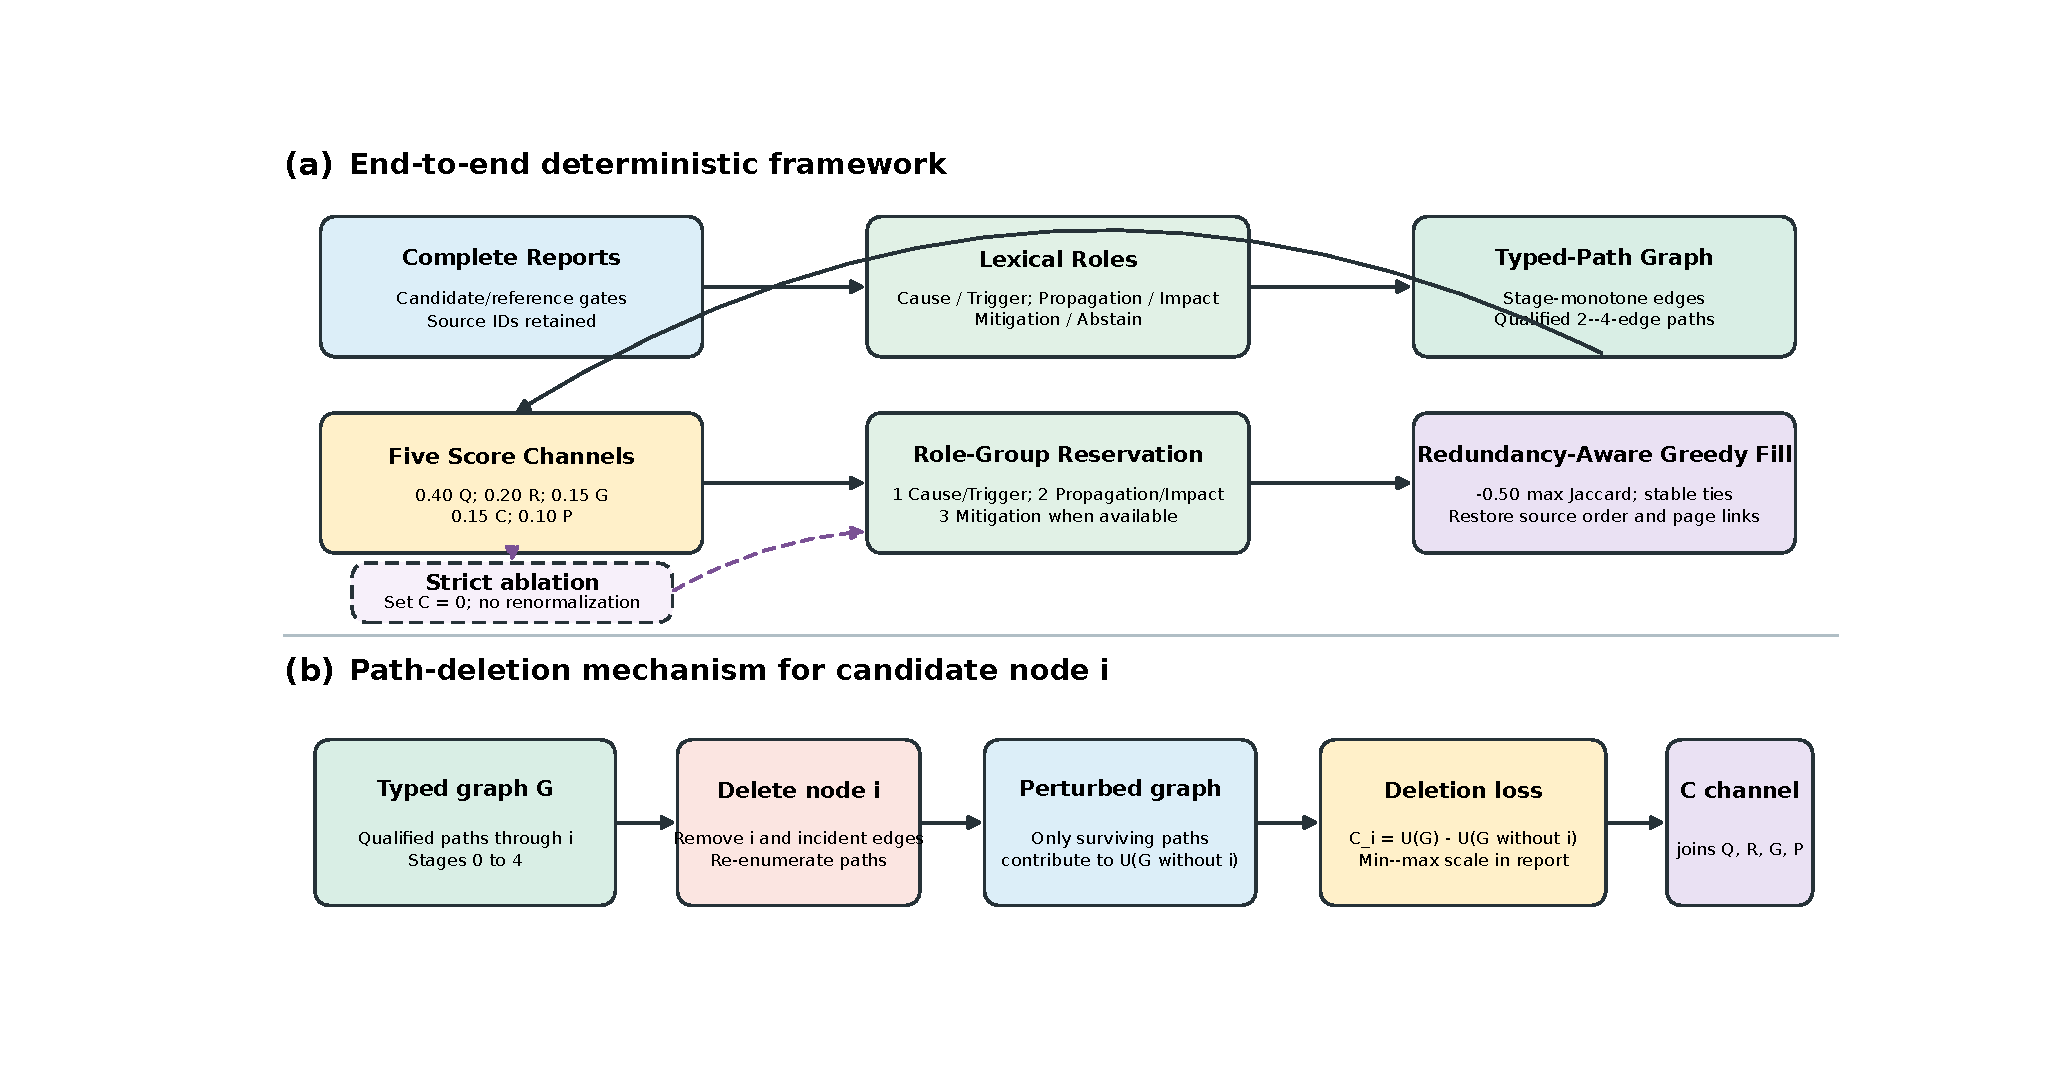
\includegraphics[width=\textwidth]{figures/fig01_algorithm_dual_panel.pdf}
\caption{Deterministic \cges{} pipeline and path-deletion mechanism. \textbf{(a)} Complete reports pass candidate and reference-separation gates; retained passages receive lexical roles and form a typed textual graph. The five score channels feed an ordered role-group reservation followed by redundancy-aware greedy filling. The unrenormalized coefficient-removal comparison sets $C$ to zero without renormalizing the remaining coefficients. \textbf{(b)} For candidate node $i$, path-deletion loss removes $i$, recomputes qualified-path utility, and takes $C_i=U(G)-U(G\setminus i)$.}
\label{fig:algorithm}
\end{figure}

The unit of analysis is the report. Candidate units within a report share topic, vocabulary, layout, and reference-summary content and are not treated as independent observations. Candidate-level quantities drive selection, whereas paired differences and composition intervals use the 15 report-level observations.

Three label families recur. AB-0 to AB-6 form the incremental component chain; RP-00, RP-10, RP-01, and RP-11 are the reservation--path $2\times2$ cells; G-U and G-T are the untyped and typed graph-salience conditions. RSI denotes the held-out matched-budget path-utility revision, and E1--E5 denote the planned external evidence stages described in Section~\ref{sec:future-validation}. Three development actions are distinguished throughout: a pre-test 144-configuration development search that selected the configuration reported in the historical comparison, a post-test 147-configuration leave-one-report-out calibration on the same 12 development reports, and a prospectively frozen 15-variant path-utility freeze whose single selected variant was then scored on the 15-report retained test.

\subsection{Corpus Construction and Reference Separation}

The corpus builder inspected 40 complete public PDFs covering 3200 declared pages. It retained 27 reports and excluded 13 before outcome computation; 12 retained reports were assigned to development and 15 to test. Figure~\ref{fig:data-flow} summarizes this construction, and Supplementary Table~S1 provides the non-verbatim sampling frame and exclusion reasons.

Inclusion required a complete readable PDF, a detectable summary reference, a non-empty post-summary candidate region, and passage of the predefined extraction-quality gates. Exclusion was decided before outcome computation and remained visible in the inventory. This procedure reduces discretionary removal after observing ROUGE values, but it also changes the estimand: the results concern reports that satisfy the builder's document and reference requirements, not every NERC publication. An operationally important report without a conventional Executive Summary remains outside the present automatic evaluation.

Development and test assignment was performed at report level so that sentences from one source could not cross partitions. Reference-summary text was used only for development scoring or final evaluation, never as a candidate. The builder preserved report ID, page interval, source order, and candidate ID so that every downstream score could be joined directly to its extraction record.

\begin{figure}[H]
\centering
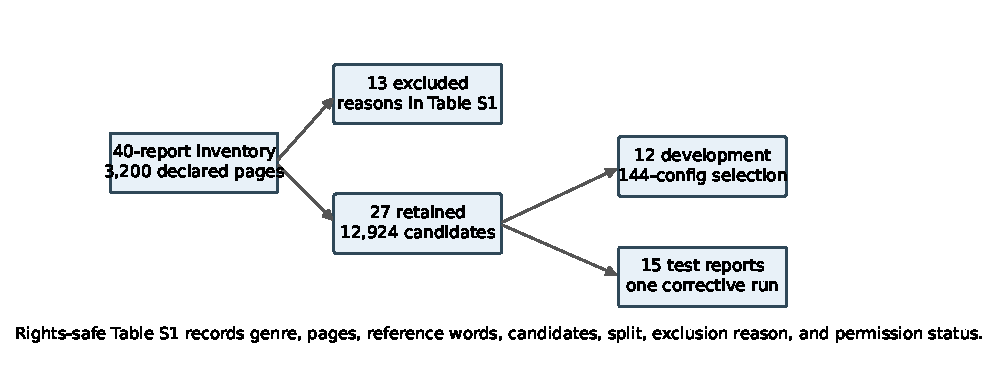
\includegraphics[width=\textwidth]{figures/fig02_dataset_flow.pdf}
\caption{Corpus construction and partitioning. Boundary and extraction-quality gates retained 27 of 40 complete PDFs. Twelve reports supported configuration selection, and 15 formed the retained test set.}
\label{fig:data-flow}
\end{figure}

Candidates begin after a conservatively detected Executive Summary boundary, and no fixed sentence cap is applied. The builder produced 12,924 candidates, with 51--1898 per report. Rebuilding the corpus found no reference/body page overlap, normalized exact candidate/reference match, or normalized common substring of at least 50 characters. These checks prevent direct reference leakage caused by page or extraction errors; legitimate paraphrase and facts repeated in the report body remain part of the task.

\subsection{Confirmatory Extension Protocol and Layout-Aware Units}

The repository also contains a machine-readable protocol for a possible confirmatory extension. It is intentionally retained as a non-executable draft because the reports used in the present pilot were accessed before a freeze and cannot be relabeled as unseen. Any future confirmatory evaluation must instead supply a new rights-cleared inventory, source-file hashes, series-disjoint development and test assignments, immutable method revisions, parameter spaces, random seeds, and a signed tuning decision before outcome access. At least eight independent external series are required and 12 are recommended; report series, rather than individual reports, would be the allocation and inferential unit. This protocol is future-work infrastructure and is not a submission claim gate for the diagnostic study reported here.

The exploratory pilot used a PyMuPDF block rule that distinguishes body paragraphs, headings, list items, table units, captions, and footnotes; removes recurrent headers, footers, and page numbers; prevents table rows from being fused with body sentences; repairs cross-line units; and stores unit type, page, coordinates, source order, word count, and tokenizer length. Three revisions were made after machine error-discovery feedback, so the resulting boundary audit is developmental rather than blinded validation. A future confirmatory study would freeze the rule only after independent boundary review and before external outcomes are accessed.

The exploratory word budgets are 110 and 260 words. Budget enforcement occurs during selection over the complete ranking: a unit that cannot fit the remaining budget is skipped, later units remain eligible, and no unit is truncated. All systems use the same candidates and budget function. Fixed $K\in\{5,10\}$ results are retained only for historical comparability.

\subsection{Sentence Roles and Typed Textual Proxy Graph}

Each candidate receives lexical evidence for root cause, trigger event, propagation or response, impact, and mitigation. Positive top-score ties lead to abstention rather than resolution by a fixed role order; all 111 development ties received no dominant role and no incident directed edge. The v0.3 selector received no reference role labels.

For each role, the implementation counts predefined cue classes and divides all non-negative scores for that role by the largest score in the report. The role channel $R_i$ is the maximum of these five unit-scaled values. A dominant role is assigned only when one positive role score is uniquely maximal. An all-zero vector or equal positive maximum yields abstention. An abstaining unit remains eligible for selection through the non-role channels but contributes no typed-path edge.

Table~\ref{tab:taxonomy} gives the executable taxonomy and representative substring-based lexical cues. The system does not detect grammatical scope, factual status, or document-level coreference.

\begin{table}[H]
\caption{Executable role and transition taxonomy. These are lexical text proxies, not expert labels or physical relations.}
\label{tab:taxonomy}\centering\small
\begin{tabularx}{\textwidth}{p{2.2cm}XX}
\toprule
Role & Representative cue classes & Permitted outgoing transitions\\
\midrule
Root cause & cause, due-to, failure, and protection-setting terms & trigger; propagation or response; mitigation\\
Trigger event & fault, outage, initiation, trip, and fire terms & propagation or response; impact\\
Propagation or response & trip, voltage, frequency, islanding, load-shed, reserve, and flow terms & impact\\
Impact & quantities with grid units, customer, load, loss, and unavailability terms & mitigation\\
Mitigation & recommendation, corrective, preventive, and standard terms & none\\
Abstention & no positive cue, or more than one equal positive maximum & none\\
\bottomrule
\end{tabularx}
\end{table}

A directed edge is allowed only for predefined stage-monotone role transitions whose candidate positions differ by at most 12. The implementation maps root cause, trigger event, propagation or response, impact, and mitigation to stages 0, 1, 2, 3, and 4, respectively. Let $d_{ij}=|\operatorname{pos}(i)-\operatorname{pos}(j)|$, let $J_{ij}$ be token-set Jaccard overlap, and let $r_i,r_j\in[0,1]$ be the unit-scaled dominant-role scores. The edge weight is
\begin{equation}
w_{ij}=\operatorname{round}_{12}\!\left[0.45\exp(-d_{ij}/5)+0.30J_{ij}+0.25\min(r_i,r_j)\right].
\label{eq:edge-weight}
\end{equation}
Thus $w_{ij}\in[0,1]$. Min--max scaled weighted degree within the report forms graph salience $G_i$.

The edge gate has semantic and positional components. The source and target roles must appear in the stage-monotone transition set in Table~\ref{tab:taxonomy}, and their candidate indices must lie within the 12-position horizon. The implementation uses absolute positional distance and therefore does \emph{not} require the source-role unit to occur earlier in document order; edge direction follows the role transition rather than chronology. The weight rewards proximity, lexical continuity, and confident role assignments. A high weight therefore means ``nearby, lexically connected, and compatible with the predefined role progression''; it does not indicate that a domain expert verified the relation or its temporal order.

These choices make the graph sparse and document specific. Sparse construction limits path enumeration and improves inspectability, while document-specific normalization avoids comparing raw node degrees across reports of very different size. The design also creates known blind spots. A causal statement whose evidence and consequence are separated by more than 12 candidates cannot form an edge; a relation expressed through coreference may have low token overlap; a role-compatible edge may point against document chronology; and a valid sentence with two equally strong role cues abstains. These are algorithmic consequences rather than post hoc explanations of individual outcomes.

\subsection{Typed Path-Deletion Structural Perturbation}
\label{sec:path-deletion}

Let $\mathcal{P}(G)$ be the set of simple, stage-monotone paths with two to four edges beginning at a root-cause or trigger node and ending at an impact or mitigation node. For path $p$,
\begin{equation}
\operatorname{strength}(p)=\left(\prod_{e\in p}w_e\right)^{1/|p|}\frac{\max\operatorname{stage}(p)-\min\operatorname{stage}(p)}{4}.
\label{eq:path-strength}
\end{equation}
The graph utility and raw deletion score are
\begin{equation}
U(G)=\sum_{p\in\mathcal{P}(G)}\operatorname{strength}(p),\qquad
C_i=U(G)-U(G_{-i})=\sum_{p\ni i}\operatorname{strength}(p).
\label{eq:deletion}
\end{equation}
Unlike weighted degree, $C_i$ depends on qualified multi-edge path membership, role order, and the geometric mean of edge weights. A synthetic unit-test counterexample gives two nodes equal weighted degree but unequal qualified-path membership. Unit tests verify deletion-loss equality, deterministic scaling, cache equivalence, and fail-closed work limits. These checks establish software and mathematical non-identity, not physical causality or effectiveness.

The functional has three design properties under a fixed qualified-path set: non-negativity when edge weights are non-negative; nullity for a node that belongs to no qualified path; and additivity over the qualified paths that contain the deleted node. More precisely, if deleting node $i$ removes exactly those paths containing $i$ and does not change the weights of paths that remain, then $C_i=\sum_{p\ni i}\operatorname{strength}(p)$. This proposition is an accounting identity for a fixed textual graph, not a causal-identification theorem. It can fail as a model of semantic influence when deletion would change role assignments, coreference, discourse interpretation, or the weights of surviving relations; the implemented perturbation intentionally holds those quantities fixed.

Table~\ref{tab:toy-path} provides a synthetic walk-through that is independent of the experimental corpus. Consider five source-ordered nodes with roles root cause, trigger, propagation, impact, and mitigation and four compatible edge weights. The four qualified paths that begin at the root-cause or trigger node and end at impact or mitigation have strengths 0.566964, 0.741559, 0.367423, and 0.542282 under Equation~\eqref{eq:path-strength}, giving $U(G)=2.218228\approx2.218$. Deleting the propagation node removes all four paths, so $C_{q}\approx2.218$; deleting the root-cause node removes only the two paths that start there, so $C_{r}=1.308523\approx1.309$. The example shows why path participation and stage span matter beyond local edge totals.

\begin{table}[H]
\caption{Synthetic typed-path example used only to explain the implemented computation; it is not an experimental observation.}
\label{tab:toy-path}\centering\small
\begin{tabular}{llll}
\toprule
Nodes on path & Edge weights & Stage-span factor & Path strength\\
\midrule
$r\rightarrow t\rightarrow q\rightarrow i$ & 0.8, 0.6, 0.9 & $3/4$ & 0.567\\
$r\rightarrow t\rightarrow q\rightarrow i\rightarrow m$ & 0.8, 0.6, 0.9, 0.7 & $4/4$ & 0.741\\
$t\rightarrow q\rightarrow i$ & 0.6, 0.9 & $2/4$ & 0.367\\
$t\rightarrow q\rightarrow i\rightarrow m$ & 0.6, 0.9, 0.7 & $3/4$ & 0.542\\
\bottomrule
\end{tabular}
\end{table}

The equality $C_i=\sum_{p\ni i}\operatorname{strength}(p)$ follows because node deletion removes exactly the qualified paths containing $i$ and leaves the remaining path strengths unchanged. The implementation recomputes or cache-checks the deleted graph, and direct deletion loss, membership-sum loss, and cached loss must agree within the numeric tolerance. The raw $C_i$ values are then min--max scaled within the report.

\subsection{Scoring and Selection}

The Full base score is
\begin{equation}
S_i=0.40Q_i+0.20R_i+0.15G_i+0.15C_i+0.10P_i,
\label{eq:full-score}
\end{equation}
where $Q_i$ is min--max scaled centroid-style lexical relevance, $R_i$ is the maximum unit-scaled role evidence, $G_i$ is min--max scaled weighted-degree salience, $C_i$ is min--max scaled path-deletion loss, and $P_i=1/(1+\operatorname{pos}(i))$ is the unrescaled positional prior for zero-based source position. Path and expansion caps are 250,000 and 2,000,000; reaching either cap terminates the computation rather than returning a partial path score.

The unrenormalized coefficient-removal comparison changes only the coefficient of $C_i$ from 0.15 to zero. It does not renormalize any remaining coefficient or alter candidates, graph construction, role-group reservation, redundancy penalty, tie rules, or budgets. Consequently, the positive-channel weight decreases from 1.00 to 0.85 while the redundancy coefficient remains 0.50; relative to the remaining positive scale, that penalty is $0.50/0.85=0.5882$, 17.6\% larger than 0.50. The primary contrast therefore estimates coefficient removal under this unrenormalized scoring rule, including relative-scale coupling, rather than a pure information-only contribution of $C_i$. A post-run clean diagnostic divides the corresponding no-path base score by 0.85, giving unit-sum remaining weights $(0.470588,0.235294,0.176471,0,0.117647)$ while retaining the 0.50 redundancy penalty and every selection rule.

Each score channel has a distinct interpretation. $Q_i$ rewards lexical terms that recur across the report and can therefore favor generic report language. $R_i$ rewards predefined condition, event, impact, and mitigation cues but is vulnerable to cue ambiguity. $G_i$ rewards local connectivity under the typed edge rules, whereas $C_i$ rewards membership in qualified paths and can differ from degree. $P_i$ favors earlier source positions. The scaling rules bound all channels to $[0,1]$ within a report but do not make their meanings interchangeable.

Selection has two phases. When $K\geq3$, the selector first considers three role groups in the fixed order (i) root cause or trigger event, (ii) propagation or response or impact, and (iii) mitigation. If a group has eligible candidates, it reserves the candidate with the largest base score. Ties use earlier source position and then sentence identifier. A group with no eligible candidate is skipped; the method never manufactures a role assignment to satisfy the reservation.

After reservation, the selector fills the remaining positions by maximizing
\begin{equation}
S_i^{\prime}=S_i-0.50\max_{j\in A}J(i,j),
\label{eq:redundancy}
\end{equation}
where $A$ is the selected set and an empty maximum is zero. Exact ties again use earlier source position and then sentence identifier. The selected set is finally reordered by source position for presentation. The role-group phase uses the base score without a redundancy penalty, so its contribution to structural coverage is separate from the path-deletion channel. No stochastic decoding or model sampling occurs in this selector.

The dominant computational cost arises from candidate-pair edge checks and bounded path enumeration. The implementation screens every ordered source--target pair, so edge construction is $O(n^2)$. The absolute 12-position gate limits admitted local ordered pairs to at most approximately $24n$ apart from boundary effects, but it is applied after the quadratic scan. Path enumeration can still grow combinatorially in a dense compatible region, which motivates the 250,000-path and 2,000,000-expansion limits.

The output is designed for source navigation. Each selected item preserves report and candidate identifiers, and a deterministic non-verbatim locator joins them to page, source order, report metadata, and source URL. All 1575 selected references resolved uniquely to an integer page within the declared PDF range, allowing readers to reopen the source page and inspect the surrounding context.

\subsection{Ablation Design and Controlled Variants}

The exploratory component study implements three controlled comparison families whose configuration registry is preserved with the results. The incremental chain begins with relevance and position (AB-0), then adds role score (AB-1), role-group reservation (AB-2), typed-graph salience (AB-3), normalized path deletion without redundancy (AB-4), and redundancy to form normalized Full (AB-5). AB-6 retains every AB-5 component except path deletion and is therefore the primary controlled path comparison. The historical unrenormalized coefficient-removal condition receives no AB identifier and remains a scale-coupled historical diagnostic.

A $2\times2$ factorial holds typed graph salience, redundancy, candidates, budgets, seeds, and tie rules fixed while independently switching role-group reservation and normalized path deletion: RP-00 disables both, RP-10 enables reservation only, RP-01 enables path deletion only, and RP-11 enables both. The analysis estimates the reservation main effect, path main effect, and their interaction. A separate G-U/G-T pair holds reservation on, path off, and redundancy on while changing only untyped versus typed graph salience. This pair isolates the net value of edge-type information from graph connectivity itself.

For every clean deletion or addition of a positive component, positive weights are renormalized to sum to one and the redundancy penalty retains the same definition relative to that positive scale. Every condition stores per-report selections, metrics, realized words, budget utilization, runtime, peak memory, failure state, configuration, seed, and code revision. Required outcomes are ROUGE-L, redundancy, role coverage, typed-edge coverage, and selection Jaccard; ROUGE alone is insufficient to interpret a structural component.

\subsection{Method Assumptions and Failure Modes}

The lexical roles are executable features rather than expert labels. Ambiguous positive ties lead to abstention, but an unambiguous cue can still assign an incorrect role. Negation scope, hypothetical or quoted events, and document-level coreference are not modeled. A transition can also join locally compatible roles without a supported discourse relation. These assumptions make the method deterministic and inspectable while limiting semantic coverage.

Errors can enter through segmentation, role assignment, edge construction, or final selection. For example, a PDF table may remain fused with prose, a candidate may receive the wrong dominant role, compatible role cues may form an unsupported edge, or a relevant extract may omit necessary context. ROUGE cannot distinguish these layers. Future expert annotation should therefore score extraction-unit validity, role or abstention, relation support, source faithfulness, and omission separately.

\subsection{Human-Validation Protocol Reserved for Future Work}
\label{sec:human-validation-protocol}

No human annotation was conducted for the reported study. The repository preserves a future-work protocol requiring two independent annotators, including at least one person with documented power-system reliability, event-analysis, or closely related technical-report experience. Its target sample comprises 200 extraction units for boundary assessment, 200 role judgments that may reuse those sampled units as a separate task, 150 typed edges, 80 complete typed paths, and 30 system-summary sets, stratified by report series, split, layout, role confidence, path availability, direction agreement, and Full/no-path selection agreement. During independent annotation, annotators would be blinded to system scores, condition names, automated role labels, and one another's labels. Recruitment and data collection require a documented institutional ethics decision before they begin.

That protocol is not the only evidence obtainable without new recruitment. Because the roles and edges are lexical constructs, the study additionally audited them against two public corpora that carry human annotation: enhanced-RST discourse relations from the Georgetown University Multilayer (GUM) corpus, and the professionally annotated intervention and outcome spans of EBM-NLP. Section~\ref{sec:construct-audit} reports what that audit shows and where it stops. It constrains how much the role and edge channels can carry and closes no row of Table~\ref{tab:e2-gate}; the reserved domain annotation remains the only evidence that can license role, edge, path, faithfulness, or omission claims.

The reserved tasks separately assess standalone unit validity; one of five roles, none/other, or ambiguous/multiple roles; edge support and direction; path coherence and information added beyond role reservation; and source faithfulness, contextual distortion, critical omission, and page-locator correctness. Until that study is independently executed, lexical roles, typed edges, and typed paths are described only as heuristic textual proxies. The two-model audit reported below is kept outside this protocol and cannot satisfy any human-validation threshold.

\subsection{Development Selection and Comparators}

The 12-report development search evaluated 144 predefined configurations. Its ordered objective maximized mean ROUGE-L F1 at $K=5$, followed by mean ROUGE-1 F1, lower redundancy, and earliest configuration order. Grid index 60 was selected, with mean development ROUGE-L F1 of 0.1195126 and ROUGE-1 F1 of 0.2713870. Full minus the unrenormalized coefficient-removal comparison was $-0.0056652$ on development.

Seven conditions share the same candidate space: Lead, lexical Centroid, TextRank, Semantic-MMR, Role, the strict graph variant without path deletion, and Full \cges{}. Semantic-MMR uses the local \texttt{sentence-transformers/all-MiniLM-L6-v2} snapshot at revision \texttt{1110a243fdf4706b3f48f1d95db1a4f5529b4d41}, with its WordPiece tokenizer, normalized embeddings, CPU execution, and Sentence-Transformers maximum sequence length of 256 tokens. It greedily maximizes the maximal-marginal-relevance objective $0.5\cos(e_i,\bar e_D)-0.5\max_{j\in A}\cos(e_i,e_j)$ \cite{carbonell1998mmr}, evaluated over the Sentence-Transformers representations \cite{reimers2019sentencebert}. Its symmetric coefficient was not optimized on development or test outcomes.

The comparators expose distinct ranking signals. Lead tests position; Centroid tests lexical representativeness; TextRank tests an untyped similarity graph; Semantic-MMR combines dense relevance and diversity; and Role tests lexical discourse evidence without graph structure. The unrenormalized coefficient-removal comparison retains the typed graph while setting the deletion coefficient to zero without renormalization. It includes the scale coupling described in Section~\ref{sec:path-deletion} rather than isolating path information alone.

Hyperparameter opportunity was not balanced for the retained-test comparison (Table~\ref{tab:tuning-opportunity}). Full \cges{} inherited a 144-configuration development search, whereas the evaluated Semantic-MMR coefficient was fixed at 0.5 and TextRank used its implementation defaults. This asymmetry is relevant to system-level ranks. RQ1 is therefore interpreted as a descriptive comparison of the reported configurations within this corpus, not as a balanced-tuning comparison of algorithms. The unrenormalized coefficient-removal comparison is the closer comparator for RQ2 because it shares the selected absolute weights, graph, candidates, and selector.

\begin{table}[H]
\caption{Tuning opportunity and inferential role. The reported intervals condition on the selected Full configuration and do not include model-selection uncertainty.}
\label{tab:tuning-opportunity}\centering\small
\begin{tabular}{p{0.25\textwidth}p{0.22\textwidth}p{0.40\textwidth}}
\toprule
Comparison object & Development opportunity & Analytical role\\
\midrule
Full \cges{} & 144 predefined configurations & Selected deterministic system; selection uncertainty omitted\\
Unrenormalized coefficient removal & Same absolute weights, $C=0$ only & Component comparator; redundancy is relatively stronger\\
Semantic-MMR & Coefficient fixed at 0.5 & Semantic relevance--diversity comparator\\
TextRank & Implementation defaults & Untyped graph-ranking comparator\\
\bottomrule
\end{tabular}
\end{table}

After the retained-test results were known, a separate development-only exercise assigned exactly nine configurations to each of Semantic-MMR, TextRank, and a normalized-path \cges{} variant under one ordered objective over both budgets. It selected Semantic-MMR coefficient 0.9, TextRank damping 0.65, and normalized path weight 0.0. The script records that it did not access the test input. These choices are reserved for a prospectively frozen external-series study and were not substituted into any retained-test result; consequently, they close the configuration-budget asymmetry only for that planned experiment, not retrospectively for RQ1.

The prospective comparator registry additionally allocates nine configurations to PacSum-MiniLM: preceding-position coefficients $-2$, $-1$, or $0$, a fixed following-position coefficient of $1$, and similarity-threshold fractions $0$, $0.3$, or $0.6$ \cite{zheng2019pacsum}. Its clean-room source and identity record are frozen in the reproducibility package; the inspected public upstream repository supplied no license file and no upstream code was copied. PacSum-MiniLM tuning and performance evaluation remain blocked until the layout boundary audit passes, so it does not appear in the historical Results.

Sentence-count budgets allow every method to return five or ten complete source units. They do not guarantee equal information because extraction units vary in length. Output length was therefore analyzed after selection as a diagnostic; the frozen primary outputs were neither truncated nor reselected. A separate post-run word-cap sensitivity, defined after the primary result was visible, is described below and remains outside the confirmatory family.

\subsection{Statistical Analysis}

For the reported post-access pilot, the primary exploratory estimand is the equal-series mean paired ROUGE-L F1 difference. Report outcomes are first averaged within \texttt{report\_series\_id}; series then receive equal weight. The system family compares no-path \cges{} with Semantic-MMR, TextRank, and PacSum-MiniLM at 110 and 260 words. The component analysis treats the AB incremental chain, reservation--path factorial, and typed--untyped graph comparison as separate families. Every key contrast reports the paired effect, a 95\% series-cluster bootstrap interval, an exact series sign-flip value, Holm adjustment within its family, and leave-one-series-out stability. These families were fixed for the v3 diagnostic run but not before source access, so their results remain exploratory. A future confirmatory study would additionally require a positive mean, an interval lower bound above zero, an adjusted exact value below 0.05, matched realized length, and no leave-one-series-out reversal before making an advantage claim.

The historical retained-test estimand is the unweighted mean report-level ROUGE-L difference on the 15-report set. Three Full-minus-baseline contrasts were defined at each budget: the unrenormalized coefficient-removal comparison, Semantic-MMR, and TextRank. Paired percentile composition intervals use 10,000 report-level resamples. For paired deltas $d_1,\ldots,d_{15}$, each resample draws 15 reports with replacement and yields mean $\bar d_b$. The archived analysis also records
\begin{equation}
t_{\mathrm{boot}}=2\min\left\{B^{-1}\sum_{b=1}^{B}\mathbb{1}(\bar d_b\leq0),\;B^{-1}\sum_{b=1}^{B}\mathbb{1}(\bar d_b\geq0)\right\},\quad B=10{,}000.
\label{eq:tboot}
\end{equation}
Because resamples are centered on the observed deltas rather than generated under a null, $t_{\mathrm{boot}}$ is a descriptive sign-tail quantity and not a calibrated hypothesis-test $p$ value. The composition intervals characterize sensitivity to the retained report set; they are not population confidence intervals. ROUGE-1, ROUGE-2, redundancy, and other pairings are descriptive \cite{cameron2008bootstrap}.

An exact paired sign-flip sensitivity enumerates all $2^{15}=32{,}768$ report-level sign assignments for each contrast and applies Holm adjustment across the six values \cite{holm1979simple}. A second post-result sensitivity maps the 15 reports to the 10 frozen \texttt{report\_series\_id} clusters, averages within each series, assigns equal weight to series, enumerates all $2^{10}=1024$ series-level sign assignments, and uses a 10,000-draw series-cluster bootstrap plus leave-one-series-out analysis. A third post-run sensitivity derives 110- and 260-word caps mechanically from development candidate lengths and greedily admits complete sentences from each archived top-10 ranking; its six Full-minus-baseline contrasts use the same equal-series bootstrap, exact series sign flip, and Holm family. None of these sensitivities is a fresh confirmatory test. The interpretation in the main text relies primarily on effect sizes and explicitly distinguishes report-level from series-level robustness.

The run contains all $15\times7\times2=210$ report--condition--budget records. Packaged checks rebuild aggregate values, contrast records, candidate boundaries, and selected source identifiers. Detailed file identities and check results are provided in Supplementary Table~S3.

\subsection{Exploratory Development-Only Calibration}

After the test result was known, a separate exploratory program evaluated 147 semantically deduplicated configurations using only the 12 development reports. It varied path-deletion weight, weight-allocation rule, path horizon, and gating rule. Twelve leave-one-report-out folds selected a zero-weight configuration in 12/12 folds. This analysis diagnoses integration behavior and was not applied to the retained test reports.

\subsection{Held-Out Matched-Budget Path-Utility Revision}

A later freeze-before-eval protocol redesigned the path channel without reading 15-test or seven-series scores for the new utilities. Five utilities (historical deletion loss, relevance-gated, end-stage weighted, length-damped, and gated-length) and three path weights (0.05, 0.10, 0.15) were scored on the 12-report development split at complete-ranking 110- and 260-word budgets. The protocol maximized the development mean of the two budgets, with documented tie-breakers. The frozen choice was the historical utility at weight 0.10. On the 12 development reports that variant scored 0.08541 and 0.12532 mean ROUGE-L at 110 and 260 words, against 0.08265 and 0.12197 for the no-path reference, so it beat that reference at both development budgets. The freeze rule selects among positive path weights, which makes no-path a development reference rather than a freeze candidate; the selected variant is scored on the 15-test whether or not it leads the reference on development. The earlier 147-configuration search and this freeze are therefore not two answers to one question: that search is post-hoc over a wider design space that includes weight-allocation, path-horizon and gating rules, and it selects a zero weight in every fold, whereas the freeze is prospective over 15 variants that all carry a positive weight, because a study of whether a redesigned path can clear the no-path reference has to freeze some path variant for the test to mean anything. That configuration, no-path \cges{}, and TextRank were then scored on the 15-report retained test at the same budgets. The 15-test run is held-out for this revision. It is not an unseen confirmatory corpus: those reports were already used in the historical evaluation, and the seen-exclusion registry contained no unused lawful public series.

\subsection{Generative-AI Assistance and Verification Boundary}

The OpenAI Codex agent interface assisted with prose drafting and editing, suggestions for experiment and audit planning, Python and \LaTeX{} development and review, provenance records, manuscript builds, and visual-quality checks. DeepSeek and Codex also independently labeled a small, fixed unit-validity and role packet to identify extraction failures during the exploratory pilot. These labels are reported only as a machine error-discovery audit: neither model was treated as a qualified power-grid expert, human annotator, or adjudicator. All ROUGE, budget, ablation, and statistical values came from documented local execution rather than generated model assertions. The authors reviewed the assisted work and retain responsibility for the study and manuscript.

\section{Results}

\subsection{Overview of Historical Empirical Findings}

The internal evidence is presented in four explicitly separated layers (Table~\ref{tab:evidence-layers}), followed by two bounded layers that are not pooled with them: an adjacent-corpus construct audit of the role and edge cues (Section~\ref{sec:construct-audit}) and a prospective frozen external evaluation on a new report family (Section~\ref{sec:external-prospective}). The primary path-component evidence is the length-controlled, normalized Full versus no-path contrast: AB-5 versus AB-6 in the seven-series factorial and the series-equal Full-minus-no-path differences of $-0.00799$ and $-0.00718$ at 110 and 260 words. The retained-test layer diagnoses the original equal-unit evaluation, where the unrenormalized coefficient-removal comparison produced the highest overall ROUGE-L mean and Full \cges{} exceeded Semantic-MMR and TextRank only under unequal information budgets; that unrenormalized contrast is a scale-coupled historical diagnostic, not the component estimand. The post-access exploratory layer tests the revised word-budget pipeline on seven additional series and supplies the controlled component diagnostics. A third layer freezes a redesigned path utility on the 12-report development split and scores the 15-report test at matched 110- and 260-word budgets; that layer is held-out for this revision, not unseen confirmatory. A fourth layer scores a four-series synthetic stress set, which exercises software and endpoint alignment on fictional fixtures rather than real-report validity. None of the four layers supports confirmatory superiority, unseen generalization, expert gold, or semantic-validity claims.

\begin{table}[H]
\caption{The six evidence layers, their resources and claim bounds. No layer supports confirmatory superiority, author-attested unseen evaluation, or expert-gold construct validity, and no two layers are pooled.}
\label{tab:evidence-layers}\centering\scriptsize
\begin{tabularx}{\textwidth}{p{2.4cm}p{1.3cm}p{2.0cm}p{3.0cm}X}
\toprule
Layer & $n$ & Budget & Main contrast & May support / may not support\\
\midrule
L1 Historical retained test & 15 reports & $K=5/10$ units & Full vs Semantic-MMR, TextRank, unrenormalized removal & Corrected wins for Full against both baselines at $K=5$, qualified by 54--63\% longer outputs; descriptive ranking, not a fair-tuning comparison. Unrenormalized removal is scale-coupled.\\
L2 Seven-series pilot and component factorial & 7 series & 110/260 words & Role evidence, reservation, typed path, and typed vs untyped graph; system contrasts vs three baselines & Exploratory length-controlled component diagnosis and system contrast; the role components are the measured effects and the path layer is not. Not unseen confirmatory and not expert gold.\\
L3 External prospective evaluation & 19 reports, two organisations & 110/260 words & Full vs no-path; TextRank vs no-path & Prospective frozen external evaluation; the corrected contrasts favour the untyped ranking and put the path channel below no-path at the larger budget. Not author-attested unseen.\\
L4 Held-out path revision (RSI) & 15 reports & 110/260 words & Redesigned path vs no-path and TextRank & Held-out-for-this-revision freeze-before-eval on already-used reports; it did not meet its bounded win. Not unseen confirmatory.\\
L5 Synthetic stress set & 8 fictional reports, 4 series & 110/260 words & Full vs no-path on planted role-chain references & Software and endpoint alignment on fictional fixtures; no Holm-adjusted path contrast is nonzero. Not real incident data.\\
L6 Adjacent-corpus construct audit & 7{,}285 relation pairs; 2{,}139 sentences & n/a & Role and edge cues vs human annotation & Adjacent-domain construct audit: cues are precise when they fire and sparse and genre-bound. Not domain expert gold.\\
\bottomrule
\end{tabularx}
\end{table}

\subsection{Post-Access Exploratory External Pilot}

Eight official reports were fixed in an exploratory inventory after source metadata or snippets had already been observed. Seven PDFs from ENTSO-E, NERC, and Transpower were acquired; the fixed NESO item returned HTTP 403 and was recorded as an acquisition failure rather than replaced. Official summary sections were separated automatically as references without human adjudication. Three rule revisions used machine unit-validity feedback to split heading--body and caption--body fusions, remove incomplete and duplicate body units, and exclude raw table rows from the main experiment. The final dataset contained seven reports in seven independent series and 58--1408 candidates per report. Because access preceded freezing and extraction rules were revised during the exploratory cycle, none of these outcomes is confirmatory.

Table~\ref{tab:external-exploratory} reports the final v3 comparison. All methods used the same candidates and complete-ranking word-budget selector; mean realized length was within 5\% of its nominal budget for every method. TextRank ranked first at 110 words, whereas no-path \cges{} ranked first at 260 words. For no-path \cges{} versus Semantic-MMR, TextRank, and PacSum-MiniLM, all six series-cluster intervals crossed zero and all Holm-adjusted exact values were 1.0. Thus the pilot does not establish a length-controlled advantage.

\begin{table}[H]
\caption{Exploratory external-series mean ROUGE-L F1 under matched word budgets ($n=7$ series). The highest observed value per budget is bold, but no predefined system contrast survived Holm adjustment.}
\label{tab:external-exploratory}\centering\small
\begin{tabular}{lrr}
\toprule
Method & 110 words & 260 words\\
\midrule
Lead & 0.1657 & 0.1643\\
Centroid & 0.1560 & 0.1678\\
TextRank & \textbf{0.1690} & 0.1796\\
Semantic-MMR & 0.1590 & 0.1751\\
Role-only & 0.1563 & 0.1687\\
No-path \cges{} & 0.1668 & \textbf{0.1844}\\
Full \cges{} & 0.1588 & 0.1772\\
PacSum-MiniLM & 0.1661 & 0.1787\\
\bottomrule
\end{tabular}
\end{table}

Full-minus-no-path ROUGE-L was $-0.00799$ at 110 words (95\% series-cluster interval [$-0.01949$, 0.00149]) and $-0.00718$ at 260 words ([$-0.01828$, 0.00147]); neither exact comparison survived Holm adjustment. Typed-minus-untyped graph effects were $+0.00139$ and $-0.00544$, with both intervals crossing zero. A final machine-only audit of 29 selected units produced 93.1\% unit-validity agreement ($\kappa=0.633$) with no malformed label from either model. Role agreement between the models was 75.9\% ($\kappa=0.698$), but their agreement with the lexical role heuristic was only 48.3\% and 65.5\%. The layout filter therefore passed this limited machine prescreen, whereas role construct validity remains unestablished.

\subsection{Exploratory Component Factorial Ablation}
\label{sec:factorial}

Table~\ref{tab:factorial-main} reports the controlled path, reservation--path, and graph-type conditions. AB-5 and RP-11 are the same normalized Full configuration; AB-6, RP-10, and G-T are the same typed no-path configuration. They are repeated to make each comparison family explicit. All conditions used identical candidates, budgets, tie rules, and evaluation code, and every one of the 182 report--condition--budget cells completed successfully.

\begin{table}[H]
\caption{Exploratory component-factorial results over seven post-access report series. The primary path-component contrast is normalized Full (AB-5) versus no-path (AB-6). R-L is ROUGE-L F1, Red. is redundancy, Role is role-group coverage, and Edge is typed-edge coverage. Coverage measures formal heuristic structure, not human-validated semantic correctness.}
\label{tab:factorial-main}\centering\scriptsize
\resizebox{\textwidth}{!}{%
\begin{tabular}{lrrrrrrrr}
\toprule
& \multicolumn{4}{c}{110-word budget} & \multicolumn{4}{c}{260-word budget}\\
\cmidrule(lr){2-5}\cmidrule(lr){6-9}
Condition & R-L & Red. & Role & Edge & R-L & Red. & Role & Edge\\
\midrule
AB-5 (Full) & 0.1588 & 0.0508 & 1.000 & 0.964 & 0.1772 & 0.0509 & 1.000 & 1.000\\
AB-6 (no path) & 0.1668 & 0.0595 & 1.000 & 0.948 & 0.1844 & 0.0747 & 1.000 & 0.984\\
\midrule
RP-00 & 0.1710 & 0.0782 & 0.667 & 0.923 & 0.1870 & 0.0781 & 0.714 & 0.982\\
RP-10 & 0.1668 & 0.0595 & 1.000 & 0.948 & 0.1844 & 0.0747 & 1.000 & 0.984\\
RP-01 & 0.1741 & 0.0571 & 0.714 & 0.931 & 0.1735 & 0.0577 & 0.762 & 0.984\\
RP-11 & 0.1588 & 0.0508 & 1.000 & 0.964 & 0.1772 & 0.0509 & 1.000 & 1.000\\
\midrule
G-U & 0.1654 & 0.0673 & 1.000 & 0.876 & 0.1898 & 0.0814 & 1.000 & 0.944\\
G-T & 0.1668 & 0.0595 & 1.000 & 0.948 & 0.1844 & 0.0747 & 1.000 & 0.984\\
\bottomrule
\end{tabular}}
\end{table}

The path term materially changed the selected evidence: mean AB-5/AB-6 selection Jaccard was 0.233 at 110 words and 0.479 at 260 words. Nevertheless, AB-5 had lower mean ROUGE-L at both budgets, and this negative direction persisted after omitting each series in turn; the 110-word LOSO estimates ranged from $-0.01062$ to $-0.00329$ and the 260-word estimates from $-0.00912$ to $-0.00238$. Thus the null-adjusted uncertainty does not arise because Full and no-path usually selected the same units.

In the factorial family, reservation increased formal role coverage to 1.0 by construction, whereas enabling path without reservation raised coverage only from 0.667 to 0.714 at 110 words and from 0.714 to 0.762 at 260 words. The path effect was positive without reservation but negative with reservation at 110 words; at 260 words it was negative in both strata. The resulting interaction was negative at 110 words and positive at 260 words, and neither interaction survived Holm correction. These budget-dependent directions do not establish either pure path failure or stable functional redundancy with reservation. Supplementary Figure~S4 visualizes the interaction, and Supplementary Table~S8 reports the complete AB-0--AB-6 chain.

Typed graph information increased formal edge coverage relative to G-U but did not show a stable ROUGE-L benefit. Mean G-T/G-U selection Jaccard was 0.221 and 0.439, confirming that edge typing changed the selections rather than acting as an inert label. The 110-word graph contrast reversed direction in two of seven LOSO analyses, whereas the negative 260-word direction was preserved in all seven. Across the 26 condition--budget groups, failure rate was zero; mean estimated runtime ranged from 0.2466 to 0.4469 seconds per report and mean Python peak memory from 1.03 to 1.49 MB, excluding the separately loaded embedding model. Full and no-path had nearly identical measured resource use, so the present implementation supplies no efficiency argument for retaining the path term.

\subsection{External Prospective Evaluation on a New Report Family}
\label{sec:external-prospective}

A separate prospective protocol evaluated the same selectors on report families the historical corpus does not contain. The inventory and every rule were frozen before any score was computed, and the corpus was acquired on 22--23 September 2026 from the public document stores of the European Network of Transmission System Operators for Electricity (ENTSO-E) and from additional North American Electric Reliability Corporation (NERC) reports; it is a frozen external corpus, not an author-attested unseen set. Because the two organisations label summary sections differently, the reference rule was generalised before scoring from the earlier Executive-Summary detector to a heading test that also admits Summary and Management Summary, and candidate units are the Markdown paragraphs that follow that section. Nineteen documents qualified after removing duplicate versions of the same incident: six ENTSO-E grid incidents (including the 2024 South-East Europe and 2025 Iberia reports), seven ENTSO-E market-coupling incidents, and six NERC reports, with 21--2,000 candidate units and 102--10,935 reference words per document.

At matched 110- and 260-word budgets the path term again failed to help, and at the larger budget it was detectably worse than omitting it: Full minus no-path was $-0.002422$ (exact sign-flip $p=0.164$) at 110 words and $-0.002906$ (interval $[-0.005605,-0.000636]$, $p=0.015625$, Holm-adjusted $p=0.046875$, negative on seven documents and positive on none) at 260 words. An untyped graph baseline that shares the candidates and the budget rule exceeded no-path at the same larger budget: TextRank minus no-path was $+0.023273$ ($p=0.158642$) at 110 words and $+0.022940$ (interval $[0.008540,0.038543]$, $p=0.008095$, Holm-adjusted $p=0.032380$) at 260 words. Within the external corpus these are the only two contrasts that survive family-wise correction, and they favour the simpler untyped ranking over the typed path channel rather than supporting it. The historical equal-unit layer contains corrected wins for Full against both baselines at the smaller budget, which the length diagnostic below qualifies; the correction-carrying evidence therefore points in different directions across layers. Supplementary Table~S10 reports the means and intervals.

\subsection{Held-Out Matched-Budget Path Revision}

Table~\ref{tab:rsi-heldout} reports the frozen redesigned-path comparison on the 15-report retained test at complete-ranking 110- and 260-word budgets ($n=15$). The frozen utility is historical path-deletion loss at weight 0.10, selected on development before these scores were written. On development it had led the no-path reference at both budgets (0.08541 against 0.08265, and 0.12532 against 0.12197), so the held-out outcome reverses a development advantage rather than extending one. The redesigned path did not meet the pre-specified bounded win of a mean at least as large as no-path \cges{} at both budgets. It was 0.0002 below no-path at 110 words (0.0652 versus 0.0654) and 0.0023 above at 260 words (0.1044 versus 0.1020). TextRank was highest at 110 words (0.0675). These complete-ranking word-budget means are a different estimand from the historical equal-unit $K=5/10$ means (Full 0.1060/0.1276; unrenormalized removal 0.1094/0.1310) and do not replace the seven-series Full-minus-no-path diagnosis ($-0.00799$/$-0.00718$; no-path 0.1844 at 260 words).

\begin{table}[H]
\caption{Held-out-for-this-revision mean ROUGE-L F1 on $n=15$ retained-test reports at matched word budgets. The redesigned path was frozen on the 12-report development split. This table is not an unseen confirmatory evaluation.}
\label{tab:rsi-heldout}\centering\small
\begin{tabular}{lrr}
\toprule
Method & 110 words & 260 words\\
\midrule
No-path \cges{} & 0.0654 & 0.1020\\
Redesigned path (historical, 0.10) & 0.0652 & 0.1044\\
TextRank & 0.0675 & 0.1031\\
\bottomrule
\end{tabular}
\end{table}

\subsection{Synthetic Stress-Test Factorial}

A four-series fictional stress set (8 reports; unused themes relative to the earlier network-calibrated fixtures) was generated locally, passed the frozen distribution gates, and was scored with the same complete-ranking 110/260-word factorial used for the post-access pilot. The extractive references were assembled from the same typed role chain that the selector can recover, so this layer tests software and endpoint alignment rather than unseen real-report validity. Table~\ref{tab:synthetic-stress} reports the means. Full \cges{} exceeded no-path at both budgets (0.3886 versus 0.3750 at 110 words; 0.3481 versus 0.3269 at 260 words). The series-equal Full-minus-no-path means were $+0.0136$ and $+0.0212$, and both Holm-adjusted exact values were 1.0. Typed-minus-untyped graph means were positive, with Holm-adjusted exact values of 0.25. These fixtures are not NERC or ENTSO-E reports, are not a human-annotated gold set, and do not replace the seven-series Full-minus-no-path diagnosis ($-0.00799$/$-0.00718$) or the 15-report held-out mixed result.

\begin{table}[H]
\caption{Synthetic-stress mean ROUGE-L F1 on $n=8$ fictional reports ($4$ series) at matched word budgets. References are extractive reconstructions of the planted role chain. This table is not confirmatory and is not real incident data.}
\label{tab:synthetic-stress}\centering\small
\begin{tabular}{lrr}
\toprule
Method & 110 words & 260 words\\
\midrule
Full \cges{} & 0.3886 & 0.3481\\
No-path \cges{} & 0.3750 & 0.3269\\
G-T (typed, no path) & 0.3750 & 0.3269\\
G-U (untyped, no path) & 0.3002 & 0.2346\\
\bottomrule
\end{tabular}
\end{table}

\subsection{Historical Retained-Test Main Comparison}

Table~\ref{tab:all-results} contains all seven conditions and four recorded metrics at both budgets. Full \cges{} exceeded Semantic-MMR and TextRank on mean ROUGE-L at each equal-unit budget but was below the unrenormalized coefficient-removal comparison. Because extraction-unit lengths differ materially, these comparisons are not controlled by word or token count. Figure~\ref{fig:aggregate} visualizes the same ROUGE-L means.

\begin{table}[H]
\caption{Macro-mean results over $n=15$ test reports at equal extraction-unit counts, not equal word counts. ``Unrenorm. removal'' denotes the unrenormalized coefficient-removal comparison, a scale-coupled historical diagnostic rather than the primary path-component estimand; that estimand is the normalized Full versus no-path contrast. Bold marks only the observed maximum ROUGE-L within a budget; underlining marks the minimum redundancy. Neither convention is an inferential conclusion.}
\label{tab:all-results}\centering\small
\begin{tabular}{llrrrr}
\toprule
$K$ & Condition & R-1 F1 & R-2 F1 & R-L F1 & Redundancy\\
\midrule
5 & Lead & 0.1633 & 0.0545 & 0.0878 & 0.0668\\
5 & Centroid & 0.1955 & 0.0457 & 0.0939 & 0.2333\\
5 & TextRank & 0.1508 & 0.0356 & 0.0806 & 0.2560\\
5 & Semantic-MMR & 0.1783 & 0.0433 & 0.0853 & \underline{0.0237}\\
5 & Role & 0.1889 & 0.0557 & 0.0934 & 0.0862\\
5 & Full \cges{} & 0.2359 & 0.0611 & 0.1060 & 0.0745\\
\cmidrule(lr){2-6}
5 & Unrenorm. removal & 0.2497 & 0.0648 & \textbf{0.1094} & 0.0798\\
\midrule
10 & Lead & 0.2617 & 0.0811 & 0.1158 & 0.0554\\
10 & Centroid & 0.2809 & 0.0683 & 0.1196 & 0.2011\\
10 & TextRank & 0.2470 & 0.0615 & 0.1156 & 0.2149\\
10 & Semantic-MMR & 0.2840 & 0.0728 & 0.1133 & \underline{0.0269}\\
10 & Role & 0.3132 & 0.0848 & 0.1257 & 0.0550\\
10 & Full \cges{} & 0.3366 & 0.0874 & 0.1276 & 0.0667\\
\cmidrule(lr){2-6}
10 & Unrenorm. removal & 0.3471 & 0.0930 & \textbf{0.1310} & 0.0746\\
\bottomrule
\end{tabular}
\end{table}

Table~\ref{tab:series-cluster} reports the post-result series-cluster sensitivity. Equal-series estimates retained the direction of every report-level contrast. For Full minus the unrenormalized coefficient-removal comparison, the series-equal mean remained negative at both budgets. For the unequal-length comparisons, the Holm-adjusted exact series-level values were 0.011719 for Semantic-MMR and TextRank at $K=5$, but 0.125000 and 0.134766 at $K=10$. Thus the larger-budget lexical contrasts were not supported by this multiplicity-adjusted series-level sensitivity, and none of these comparisons resolves the length mismatch.

\begin{table}[H]
\caption{Post-result series-cluster sensitivity for Full-minus-baseline ROUGE-L differences. The 15 reports form 10 frozen series. Intervals are percentile cluster-bootstrap intervals over equal-weighted series; exact values enumerate all 1024 series sign assignments and are Holm-adjusted across six contrasts. This analysis is exploratory.}
\label{tab:series-cluster}\centering\small
\begin{tabular}{llrrrr}
\toprule
$K$ & Baseline & Series-equal mean & 95\% cluster interval & Exact $p$ & Holm $p$\\
\midrule
5 & Unrenorm. removal & -0.005744 & [-0.015986, 0.002230] & 0.316406 & 0.316406\\
5 & Semantic-MMR & 0.021864 & [0.015484, 0.028248] & 0.001953 & 0.011719\\
5 & TextRank & 0.028557 & [0.019927, 0.038486] & 0.001953 & 0.011719\\
10 & Unrenorm. removal & -0.004773 & [-0.010494, -0.000084] & 0.091797 & 0.183594\\
10 & Semantic-MMR & 0.014205 & [0.003626, 0.023764] & 0.031250 & 0.125000\\
10 & TextRank & 0.011010 & [0.001883, 0.019764] & 0.044922 & 0.134766\\
\bottomrule
\end{tabular}
\end{table}

\begin{figure}[H]
\centering
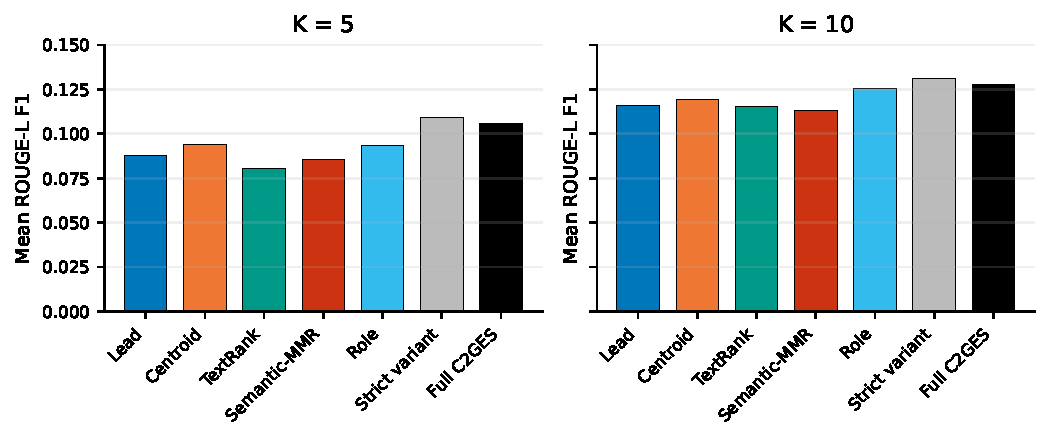
\includegraphics[width=\textwidth]{figures/fig03_aggregate_rougel.pdf}
\caption{Mean Executive-Summary ROUGE-L F1 for the seven conditions ($n=15$ reports) at equal sentence counts but unequal word counts. Bars are descriptive macro-means; paired distributions appear in Figure~\ref{fig:paired}.}
\label{fig:aggregate}
\end{figure}

Increasing the budget from five to ten units raised mean ROUGE-L for every condition, as expected when more source content is admitted. The ordering differed across methods: Role moved from 0.0934 to 0.1257 and became the strongest non-graph comparator at $K=10$, whereas Centroid was the strongest non-graph comparator at $K=5$. Results at only one extract length would therefore incompletely characterize these systems. The larger budget is not necessarily operationally preferable because brevity, coverage, and omission risk may be valued differently.

The unrenormalized coefficient-removal comparison had the largest observed ROUGE-1, ROUGE-2, and ROUGE-L mean at both budgets. Semantic-MMR had the lowest redundancy, consistent with its explicit diversity objective and shorter outputs. Full \cges{} reduced redundancy relative to the unrenormalized comparison at both budgets while also reducing all three ROUGE means. The two configurations therefore occupy different observed overlap--redundancy operating points; this result does not show that path deletion improves a joint objective.

\subsection{Historical Output-Length Diagnostic}
\label{sec:output-length}

A post-selection script counted Unicode whitespace-delimited words and characters in every selected unit. Supplementary Table~S2 contains all 14 condition--budget groups and per-report records. Table~\ref{tab:length-audit} shows the four conditions used in the main interpretation. The long-unit and Table-marker counts are selection instances, so an item selected by more than one condition or budget is counted in each output.

\begin{table}[H]
\caption{Descriptive output-length diagnostics. ``$>100$'' counts selected-unit instances longer than 100 words; ``Table'' counts units containing the exact case-sensitive string.}
\label{tab:length-audit}\centering\small
\resizebox{\textwidth}{!}{%
\begin{tabular}{llrrrrr}
\toprule
$K$ & Condition & Mean words & Mean characters & $>100$ & Table & Maximum words\\
\midrule
5 & Full \cges{} & 287.7 & 1843.6 & 12 & 14 & 140\\
5 & Unrenorm. removal & 329.0 & 2099.9 & 15 & 16 & 270\\
5 & Semantic-MMR & 184.7 & 1242.1 & 5 & 9 & 138\\
5 & TextRank & 177.0 & 1125.1 & 1 & 7 & 124\\
10 & Full \cges{} & 568.9 & 3619.5 & 25 & 26 & 270\\
10 & Unrenorm. removal & 596.9 & 3822.5 & 28 & 26 & 270\\
10 & Semantic-MMR & 354.5 & 2361.2 & 7 & 16 & 138\\
10 & TextRank & 369.0 & 2329.7 & 4 & 18 & 130\\
\bottomrule
\end{tabular}}
\end{table}

Figure~\ref{fig:length} makes the output-length mismatch visible. At $K=5$, Full used 56\% more words than Semantic-MMR and 63\% more than TextRank on average; at $K=10$, the corresponding increases were 61\% and 54\%.

\begin{figure}[H]
\centering
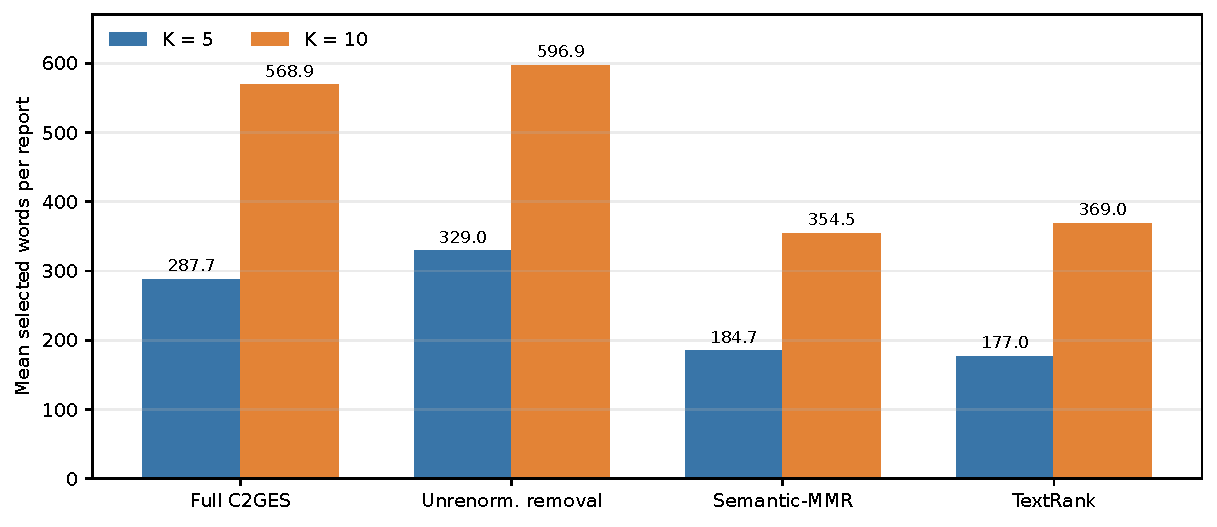
\includegraphics[width=0.90\textwidth]{figures/fig05_output_length.pdf}
\caption{Mean selected words per test report for the four principal conditions. Values reproduce Table~\ref{tab:length-audit}; no word-budget reselection was performed.}
\label{fig:length}
\end{figure}

Full averaged 103.0 and 214.5 more words than Semantic-MMR at $K=5$ and $K=10$, and 110.7 and 199.9 more than TextRank. Among its 225 selected-unit instances, 37 were longer than 100 words, 40 contained ``Table'', and the maximum was 270 words. These diagnostics show fused table, heading, footnote, or line-break blocks among the candidate extraction units. The higher historical ROUGE values relative to Semantic-MMR and TextRank are consequently equal-unit but unequal-word comparisons and do not establish a fair length-matched advantage. They motivated the explicitly post-run word-cap sensitivity in Table~\ref{tab:matched-word}.

A future confirmatory word-budget study must specify the budget before ranking, define how partially fitting units are handled, and apply an equivalent constraint to every comparator. Truncating the present outputs would answer a different question because it could cut a technical statement mid-clause and would preserve any advantage obtained while ranking long fused units.

For the post-run sensitivity, the median word totals of the first five and ten development candidates were 113.5 and 260.0; rounding to the nearest ten fixed caps of 110 and 260 words. Each method's archived top-10 ranking was traversed once, admitting only complete sentences that fit the remaining cap and then restoring document order. This reduced mean realized-length differences: at 110 words, condition means ranged from 100.5 to 105.6 words; at 260 words, they ranged from 234.1 to 249.9. The analysis nevertheless searches only the frozen top-10 pool and was designed after test outcomes were known.

\begin{table}[htbp]
\caption{Post-run matched-word sensitivity using equal-weight report-series estimands. The 15 reports form 10 frozen series. Intervals use 10,000 series bootstrap draws; exact values enumerate all 1024 series sign assignments and are Holm-adjusted across six contrasts.}
\label{tab:matched-word}
\centering\small
\resizebox{\textwidth}{!}{%
\begin{tabular}{rllrr}
\toprule
Word cap & Contrast & Equal-series difference & Cluster-bootstrap 95\% interval & Holm $p$\\
\midrule
110 & Full $-$ unrenorm. removal & +0.0020 & [$-0.0002$, 0.0041] & 0.796875\\
110 & Full $-$ Semantic-MMR & +0.0019 & [$-0.0034$, 0.0079] & 1.000000\\
110 & Full $-$ TextRank & $-0.0008$ & [$-0.0066$, 0.0046] & 1.000000\\
260 & Full $-$ unrenorm. removal & $-0.0015$ & [$-0.0072$, 0.0021] & 1.000000\\
260 & Full $-$ Semantic-MMR & +0.0062 & [$-0.0006$, 0.0142] & 0.796875\\
260 & Full $-$ TextRank & +0.0001 & [$-0.0065$, 0.0059] & 1.000000\\
\bottomrule
\end{tabular}}
\end{table}

All six intervals cross zero and no exact comparison survives Holm adjustment. Thus the top-10 word-cap sensitivity supplies no multiplicity-adjusted evidence for a Full advantage over any of the three principal comparators. Because it was post-run and does not rank beyond the archived top ten, it narrows the length concern but cannot replace a prospectively frozen matched-budget experiment.

The long-unit counts locate a concrete extraction risk. Units exceeding 100 words and units containing ``Table'' show that PDF layout sometimes survives the sentence splitter as one selectable block. Such blocks can contain many reference-summary tokens and thereby increase ROUGE without providing a concise sentence. They may remain useful source locators, but they weaken sentence-budget comparisons and motivate layout-aware segmentation before external validation.

A nonverbatim post-result extraction audit subsequently applied PyMuPDF block coordinates to all 27 included PDF files, with every source hash matching the frozen ledger. The rule preserved page/block boundaries, excluded recurrent margin material, and removed blocks overlapping detected tables by at least 25\%. It detected 505 table regions with zero page-level detection failures and produced 14,290 candidate units, of which 9824 were exact normalized matches to the 12,924 legacy units. The number of candidates exceeding 100 words decreased from 214 in the legacy pool to 39 under the block-preserving rule. This is an extraction-boundary diagnostic, not a performance result: candidates and references were not ranked or scored, and one retained block still reached 522 words. Hashed first, median, and longest-unit audit rows support manual checking without redistributing report text.

A post-run tokenizer audit measured all 12,924 development and test candidates without truncation to quantify exposure to the frozen encoder limit. Median length was 33 tokens, the 95th percentile was 89, and 38 candidates (0.294\%) exceeded 256 tokens. On the retained test split, 29 of 9504 candidates (0.305\%) exceeded 256 and the maximum was 525. A subsequent representation sensitivity first reproduced every frozen production Semantic-MMR selection and metric, then compared the same model with a 512-token limit and with 254-content-token chunk embeddings averaged only for over-limit candidates. The 512-token variant changed 0/15 reports at $K=5$ and 2/15 at $K=10$; chunk averaging changed 1/15 and 2/15. Equal-series ROUGE-L changes ranged from $-0.00057$ to $+0.00058$, and all four exact series comparisons had Holm-adjusted $p=1.0$. These tested alternatives had limited impact on this retained corpus, but they were defined post-run and do not establish general truncation robustness or identify a preferred long-text representation.

\subsection{Historical Endpoint Contribution of the Path-Deletion Term}

Table~\ref{tab:contrasts} gives the six predefined contrasts. Full minus the unrenormalized coefficient-removal comparison was $-0.003332$ at $K=5$ and $-0.003360$ at $K=10$; both report-composition intervals crossed zero. Full had slightly lower redundancy than the unrenormalized comparison (0.0745 versus 0.0798 at $K=5$ and 0.0667 versus 0.0746 at $K=10$), but redundancy was a descriptive secondary outcome. Under the current integration, the path-deletion term therefore did not improve the predefined lexical-overlap endpoint.

Full also exceeded Semantic-MMR and TextRank at both equal-unit budgets on this split. These paired differences describe the selected reports but retain the output-length mismatch documented in Section~\ref{sec:output-length}. No minimum important difference or qualified-reader outcome was specified, so the automatic contrasts do not establish practical benefit for maintenance review.

The post-run clean normalized ablation reproduced every archived Full and unrenormalized coefficient-removal selection before constructing the new comparator. Normalization changed that selection on 1/15 reports at $K=5$ and 3/15 at $K=10$. Full minus normalized no-path was $-0.00613$ and $-0.00393$ under equal-series weighting; the series-cluster intervals were [$-0.01591$, 0.00166] and [$-0.01006$, 0.00104], and both Holm-adjusted exact values were 0.441406. This same-corpus diagnostic separates path removal from the 0.85 positive-score scale but still supplies no multiplicity-adjusted evidence that the path term improves ROUGE-L.

\begin{table}[H]
\caption{Predefined Full-minus-baseline Executive-Summary ROUGE-L contrasts paired by test report ($n=15$). Intervals describe sensitivity of the mean paired difference to the composition of the retained reports. The final column is a descriptive bootstrap sign-tail quantity rather than a calibrated hypothesis-test $p$ value.}
\label{tab:contrasts}\centering\small
\begin{tabular}{llrrr}
\toprule
$K$ & Baseline & Mean difference & 95\% comp. interval & Unadjusted $t_{boot}$\\
\midrule
5 & Unrenorm. removal & -0.003332 & [-0.010889, 0.002826] & 0.3544\\
5 & Semantic-MMR & 0.020737 & [0.012765, 0.028354] & 0/10,000 tail draws\\
5 & TextRank & 0.025438 & [0.017542, 0.033722] & 0/10,000 tail draws\\
10 & Unrenorm. removal & -0.003360 & [-0.008306, 0.001040] & 0.1444\\
10 & Semantic-MMR & 0.014360 & [0.006082, 0.022215] & 0.0008\\
10 & TextRank & 0.012029 & [0.004397, 0.019241] & 0.0022\\
\bottomrule
\end{tabular}
\end{table}

Figure~\ref{fig:paired} shows every report-level difference. Full and the unrenormalized coefficient-removal comparison selected different candidate sequences in 28 of 30 report--budget cells, and their base scores differed in all 30. The coefficient rule was therefore active, although activity alone does not indicate a benefit.

\begin{figure}[H]
\centering
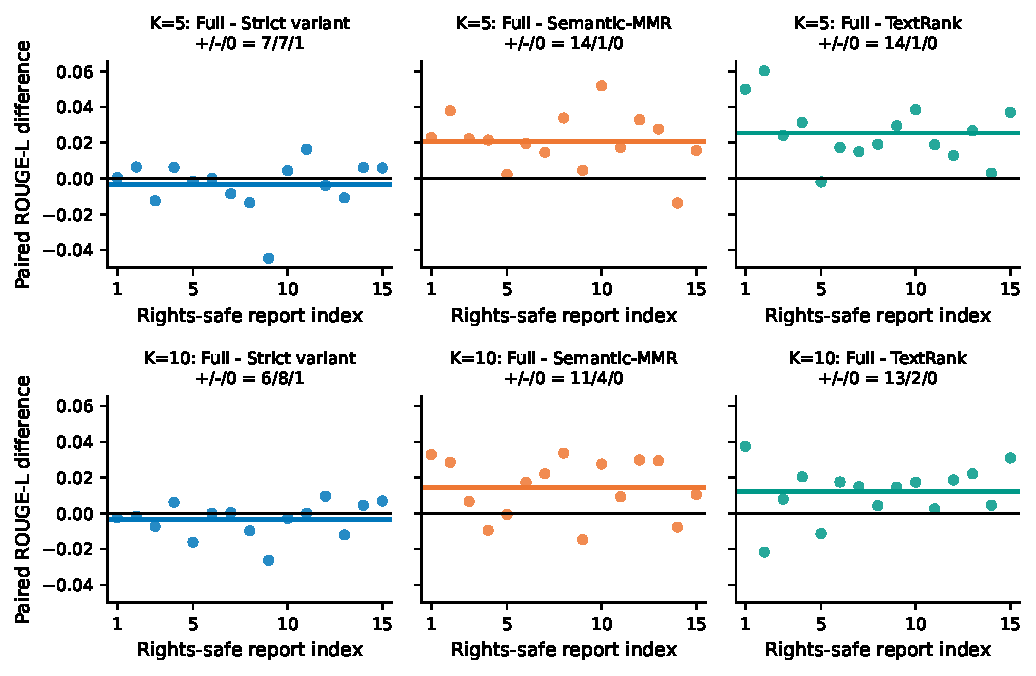
\includegraphics[width=\textwidth]{figures/fig04_paired_differences.pdf}
\caption{Per-report paired Executive-Summary ROUGE-L differences for the six predefined contrasts ($n=15$). Horizontal colored segments denote means; black lines denote zero; panel titles give positive/negative/zero sign counts. Rights-safe report indices map to non-verbatim metadata in Supplementary Table~S1.}
\label{fig:paired}
\end{figure}

The report-level signs show heterogeneity hidden by the means. Against the unrenormalized coefficient-removal comparison, Full was positive and negative on equally many non-tied reports at $K=5$ and negative on more reports at $K=10$. Against Semantic-MMR and TextRank, positive differences predominated, although the length mismatch remains. Report-level and series-level sign-flip sensitivities produced the same directions under their respective sign-exchangeability assumptions, but the multiplicity-adjusted series-level values did not support the $K=10$ baseline contrasts. Full report-level values are in Supplementary Table~S4; the series-level machine-readable analysis is included with the reproducibility files.

\subsection{Historical Component Behavior and Coefficient Support}

Across 19,008 Full/unrenormalized-removal candidate-score comparisons, 9774 were nonzero, and selected sequences changed in 28 of 30 report--budget cells. The term was therefore numerically active. Its report-level effect was heterogeneous, and the endpoint comparison in Section~\ref{sec:factorial} did not show an average ROUGE-L gain.

The post-result development-only calibration evaluated 147 semantically deduplicated configurations. A zero path-deletion weight won all 12 leave-one-report-out folds. The best nonzero candidate used weight 0.025, won no fold, and remained below its zero-coefficient comparison at both budgets. The separate equal-nine development exercise likewise selected normalized path weight 0.0 while selecting Semantic-MMR coefficient 0.9 and TextRank damping 0.65 for a future external-series protocol. Neither exercise was applied to the retained test. Together they make a simple coefficient adjustment an unpromising explanation for the negative ablation, but they cannot replace an untouched comparison. A revised component will likely require different path semantics, role evidence, or score integration.

Maximum path expansions were 19,638 of the 2,000,000 cap, and qualifying paths were 16,182 of 250,000. The selected reports were therefore processed without approaching the work limits. These observed margins describe the present corpus rather than asymptotic scalability.

\subsection{Adjacent-Corpus Construct Audit of Role and Edge Evidence}
\label{sec:construct-audit}

Role and edge evidence rests on lexical cues, so those cues were audited against two public human-annotated corpora, each obtained from its original distributor and neither redistributed. On the Georgetown University Multilayer enhanced-RST corpus, across 64 documents and 7,678 elementary discourse units the deterministic rule assigned a dominant role to 349 units (4.55\%), and among 7,285 human-annotated relation pairs only 45 (0.62\%) carried role evidence on both units, so no admissible typed edge was produced and neither precision nor recall is estimable. On the professionally annotated EBM-NLP spans, across 191 abstracts and 2,139 sentences, 382 sentences (17.9\%) received a dominant role; the mapped roles matched expert intervention spans with precision 0.610 and recall 0.064 against a 0.524 base rate, and expert outcome spans with precision 0.807 and recall 0.060 against 0.519 (Supplementary Table~S9). The cues are precise when they fire and sparse and genre-bound in general text. This adjacent-corpus audit constrains how much the role and edge channels can carry; it is not the domain adjudication reserved in Section~\ref{sec:human-validation-protocol}.

\subsection{Implementation Reliability}

All reported selections and aggregate values were reproduced from the archived run artifacts. Candidate boundaries, condition--budget completeness, source identifiers, path-work limits, and aggregate recalculation passed the packaged checks. These tests support the integrity of the reported experiment. The packaged reproducibility records contain the complete matrix, file identities, and corrective history, with key checks summarized in the Supplementary Materials.

\section{Discussion}

\subsection{Main Findings and System-Level Comparison}

The role-conditioned layers are not uniformly informative. Role evidence and role-group reservation are the components with measurable effects, and the cues behind them matched professionally annotated intervention and outcome spans at precision 0.610 and 0.807 against base rates near 0.52; the length-controlled, normalized Full versus no-path contrast shows where the same design does not pay. In the seven-series factorial, AB-5 (normalized Full) remained below AB-6 (no-path) at both 110- and 260-word budgets, with series-equal Full-minus-no-path differences of $-0.00799$ and $-0.00718$. No predefined system contrast versus TextRank, Semantic-MMR, or PacSum-MiniLM survived Holm adjustment. The historical equal-unit comparison is mixed and is not the component estimand: Full \cges{} recovered more Executive-Summary wording than Semantic-MMR and TextRank at $K=5/10$, but its outputs contained 54--63\% more words, and the unrenormalized coefficient-removal comparison is a scale-coupled historical diagnostic. A prospectively frozen path revision scored 0.0652/0.1044 against no-path 0.0654/0.1020 on the same 15 reports; it did not meet its bounded win and is held-out for this revision, not unseen confirmatory. Taken together, these results do not establish a system-level advantage and instead favor no-path \cges{} as the simpler provisional configuration. The external prospective evaluation points the same way and adds one contrast the internal studies never produced: on the new corpus the typed path channel fell below no-path at 260 words after family-wise correction, while TextRank exceeded it, so the corrected external contrasts favour the untyped ranking over the typed path, while the historical equal-unit layer still contains corrected wins for Full against both baselines at the smaller budget. Correction-carrying system evidence therefore points in different directions across layers instead of supporting one method.

\subsection{Why the Path-Deletion Term Did Not Improve ROUGE-L}

The controlled factorial changes the interpretation of the negative component result. The path term was not inert: AB-5 and AB-6 had low-to-moderate selection overlap, and Full remained below no-path in every leave-one-series-out rerun. The problem is therefore not that the implementation silently ignored the feature. Rather, path participation redirected selection toward units that increased formal path or edge coverage without improving Executive-Summary overlap. This distinction matters because a no-effect implementation bug and an active but endpoint-misaligned mechanism require different remedies; Figure~\ref{fig:component-diagnostic} summarises how many sentence scores and report--budget selections the term actually changed.

Role-group reservation remains one plausible source of overlap, because it already requires available evidence from condition/trigger, propagation/impact, and mitigation groups before ordinary greedy filling. The $2\times2$ results, however, do not establish stable redundancy: at 110 words the path effect changed from positive without reservation to negative with reservation, whereas at 260 words it was negative in both strata, and neither interaction survived family-wise correction. The defensible conclusion is therefore narrower: reservation and path can interact in a budget-dependent manner, but the seven-series pilot cannot identify a stable substitutive relationship.

Score integration is a second issue. The path channel competes with relevance and graph salience after report-level scaling. In the historical strict removal, deleting its positive weight also left the fixed redundancy penalty relatively stronger; this scale coupling motivated the normalized comparison. Because the normalized result was still negative, rescaling alone does not explain the outcome.

Lexical roles create a second limitation. Negation, hypothetical language, quotations, and cross-unit coreference are not resolved, and an edge is permitted by role compatibility and local distance rather than by expert-validated discourse relations. A candidate can therefore participate in a strong typed path without adding useful Executive-Summary wording. Conversely, a semantically important passage can receive low path participation when its related evidence lies beyond the 12-position horizon. These hypotheses are compatible with the active but heterogeneous score changes, but targeted evaluation is needed to distinguish among them.

\begin{figure}[H]
\centering
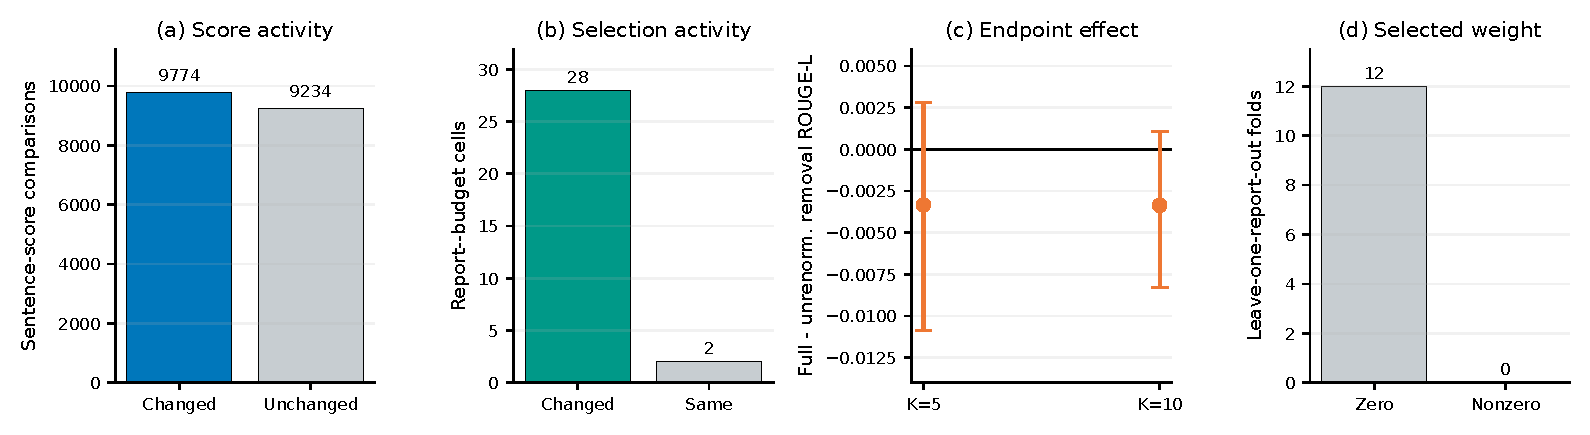
\includegraphics[width=\textwidth]{figures/fig06_component_diagnostic.pdf}
\caption{Component diagnosis for the path-deletion term. The term altered 9774 of 19,008 sentence scores and 28 of 30 report--budget selections, but Full-minus-strict-variant ROUGE-L was slightly negative at both budgets and zero weight was selected in all 12 development leave-one-report-out folds. Error bars in panel (c) are report-composition intervals.}
\label{fig:component-diagnostic}
\end{figure}

\subsection{Methodological Lessons for Structure-Aware Long-Document Extraction}

The negative component result has value beyond this implementation only if it yields testable design lessons. First, structural complexity must be evaluated incrementally: a richer graph is not supported merely because it changes rankings or improves an internal coverage score. Its contribution must be isolated against a normalized comparator and judged on a task endpoint or an independently validated structural endpoint. Second, hard coverage constraints and soft structural scores should be crossed factorially. Testing either mechanism only inside a full system can conceal substitution, antagonism, or budget dependence. Third, automatically typed edges require a construct-validity study; formal typed-edge coverage cannot be interpreted as semantic coherence when the types originate from lexical rules. Fourth, matched information budgets are essential in long-document extraction because equal sentence counts can reverse the apparent system ranking by allowing methods to emit different amounts of text.

These lessons define a falsifiable redesign path. A revised path mechanism should use expert-validated relations or uncertainty-aware role probabilities, avoid rewarding unsupported chains, and be frozen before evaluation on untouched series. It should be retained only if it improves either a prospectively declared task endpoint or a human-validated structure endpoint without unacceptable redundancy or cost. Otherwise, the simpler no-path selector is the appropriate default. This turns the failed component from a claim of hidden superiority into a documented boundary condition for future structure-aware summarization work. Stated as an information result rather than an engineering one, the exploratory comparison did not establish that role typing contributes discriminative information beyond the untyped graph: the typed-minus-untyped effects did not agree in sign across the two budgets and both intervals crossed zero. That is a failure to demonstrate added information, not a demonstration of redundancy; no equivalence test was run, and the redesign path below must be read against that weaker claim.

\subsection{Engineering Use and Source-Linked Navigation}

The intended practical role of \cges{} is to provide a structured, source-linked entry point into long reports. A reader can begin with passages associated with condition, event, impact, and mitigation roles and then return to their original pages. Deterministic selection also makes changes attributable to explicit feature channels rather than generation variability. This combination supports method development and analyst-facing prototypes, although automatic reference overlap is not a substitute for engineering judgment.

NERC reliability and disturbance reports can support lessons-learned review, but work orders and inspection records differ in vocabulary, length, asset granularity, narrative structure, and available reference summaries. An operational study would also need asset-specific terminology, access controls, abstention rules for extraction failures, and explicit evaluation of missed hazards. The current experiment establishes a technical-report workflow, not maintenance effectiveness.

\subsection{Limitations}

The test set contains 15 selected public reports from one organization, and the reports were inspected during corrective reconstruction. A post-result sensitivity grouped them into 10 frozen report-series clusters, but it cannot eliminate recurring institutional language, near-duplicate passages, or dependence between nominally distinct series. Both report- and series-level estimates therefore describe the retained corpus rather than population-wide uncertainty.

Equal sentence counts produced unequal word counts, and some extraction units retained table, heading, footnote, or line-break material. The post-run word-cap analysis equalized caps only within frozen top-10 rankings and cannot remove this extraction-boundary bias. The block-preserving extraction audit reduced long-unit incidence but was not used to rerun ranking or obtain human validity judgments. The 512-token and chunk-mean Semantic-MMR diagnostics changed few selections, but both are same-corpus post-run checks. Semantic-MMR used a fixed coefficient of 0.5 in the retained-test run, whereas \cges{} inherited a 144-configuration development search, so historical tuning opportunities were asymmetric. The later equal-nine development exercise supplies budget-matched candidate configurations only for a future external-series study. A fairer system comparison still requires prospectively frozen layout-aware units, equal word or token budgets, comparable development resources, and untouched evaluation data.

The method lacks expert role labels and expert assessment of source faithfulness, structural coverage, unsafe omission, and reading utility. ROUGE and redundancy cannot provide these judgments. The exploratory external references were extracted automatically, the source inventory was not unseen when its rules were established, one fixed report could not be acquired, and only seven series were available. The freeze-before-eval path revision uses the same 15 retained-test reports as a held-out split for this revision; it is not an unseen confirmatory corpus. The eight-report synthetic factorial uses fictional fixtures and planted extractive references; it is a software stress check, not real incident evidence. The two-model audit improved boundary-error detection but cannot establish construct validity; its limited agreement with lexical roles reinforces this restriction. The adjacent-corpus construct audit of Section~\ref{sec:construct-audit} narrows that uncertainty without removing it: the cues are precise when they fire but recover only about 6\% of professionally annotated role-bearing sentences in an adjacent domain, and produce no admissible typed edge on a corpus carrying human discourse relations. Domain expert adjudication therefore remains the only route to the reserved construct claims. Third-party licensing also prevents public redistribution of the source PDFs and verbatim derived text; non-verbatim metadata, configurations, aggregate results, code, and page locators can still be provided for review.

This diagnostic round does not complete several requested extensions. A 20--30-case expert evaluation of extract validity, role correctness, and faithfulness is reserved for E2 and requires an institutional ethics determination plus two independent annotators before recruitment; no such labels were collected here, and machine audits are not expert gold. Tuned PacSum variants and STAS were not scored on the retained 15-test; PacSum-MiniLM appears only in the post-access pilot, and adding those systems after historical outcomes were visible would remain a post-result comparison, not a confirmatory one. The 12-position edge window and non-chronological directionality are declared blind spots; they were not rescanned on the already-accessed corpora. Rhetorical Structure Theory (RST) or elementary-discourse-unit graphs and weakly supervised role classifiers were not implemented. Embedding overlap or natural-language-inference metrics such as BERTScore were not added as construct-validity substitutes for expert faithfulness or omission judgments.

\begin{table}[H]
\caption{The annotated-study gate behind every construct claim in this paper. No row is closed by the present revision.}
\label{tab:e2-gate}\centering\small
\begin{tabular}{p{0.28\textwidth}p{0.64\textwidth}}
\toprule
Precondition & State and closing condition\\
\midrule
Rights-cleared unseen series (E1) & Not established. The seven pilot series were accessed before freezing, and the seen-exclusion registry holds no unused lawful public series; closing requires an author attestation of prior non-inspection plus an inventory frozen before access.\\
Independent annotators (E2) & Not recruited. Two annotators are required, at least one with documented power-system reliability or event-analysis experience, blinded to system scores, condition names, automated role labels, and one another.\\
Institutional ethics determination & Not obtained. Recruitment and data collection may not begin before the responsible institution issues an approval, an exemption, or a formal decision that the work is not human-subjects research.\\
\midrule
May not be claimed before closure & Expert gold; construct validity of lexical roles, typed edges, or typed paths; semantic-faithfulness or critical-omission estimates; system superiority; and operational or maintenance benefit.\\
\bottomrule
\end{tabular}
\end{table}

\subsection{Future Validation}
\label{sec:future-validation}

The next evidence cycle is now specified rather than left as a general recommendation; Table~\ref{tab:e2-gate} states the gate that keeps every construct claim open until it closes. E1 freezes a rights-cleared unseen-series corpus, promotes the audited block/page rule only after boundary review, balances development opportunity---including symmetric tuning budgets for comparators and a development-selected redundancy coefficient---and compares complete-ranking outputs at 110 and 260 words. Any tuned PacSum, STAS, or other unsupervised comparator belongs in that freeze-before-access design, not as a post-result overlay on the retained 15-test. The 12-position horizon and chronological-direction rule, if revised, must be frozen before E1 outcomes are opened. E3 runs the AB-0--AB-6 chain, the reservation--path $2\times2$ factorial, and the G-U/G-T graph-type comparison on the same candidates and series split. The path component is not redesigned after external outcomes are visible; the protocol instead diagnoses whether its effect is absent, redundant with reservation, or confined to structural coverage. If a path channel is retained in that redesign, a pre-frozen candidate is a two-stage selector in which role-group reservation secures coverage and the path term acts only as a tiebreaker, isolating its contribution from additive channel competition.

E2 uses independent, blinded judgments to evaluate unit validity, roles, relations, paths, source faithfulness, and omissions. Agreement is reported before adjudication, and failed construct thresholds force claim downgrading. RST or elementary-discourse-unit graphs and weakly supervised role labels are E2-conditional alternatives, not substitutes for the missing expert gold in this round. Embedding overlap or NLI metrics such as BERTScore, and rank-aware gains with an explicit redundancy penalty such as redundancy-aware Sem-nCG \cite{akter2024semncg}, may be reported as descriptive companions after E2, but they do not close construct validity. A license-cleared corpus of maintenance narratives or work orders remains a separate conditional E5 application test. Expert task utility is likewise a separate E4 study and is required before any claim about review time, task accuracy, or unsafe omission. Neither E4 nor E5 is implied by successful completion of E1--E3.

\section{Conclusions}

\cges{} is a deterministic, role-conditioned framework for extracting source-linked passages from long power-system technical reports. Its diagnostic evaluation separates a role layer that carries measurable effects from a typed path layer that does not. Role evidence raised ROUGE-L by 0.0186 at 260 words in the pilot, and its cues matched expert-annotated spans at precision 0.610 and 0.807, while no path configuration improved the endpoint. First, the primary path-component evidence is the length-controlled, normalized Full versus no-path contrast: in the seven-series pilot, Full remained below no-path by 0.00799 and 0.00718 ROUGE-L at 110 and 260 words, and no predefined system contrast survived Holm adjustment. The path-deletion term changed candidate scores and selected sequences without improving that endpoint, and development-only calibration selected zero path weight in all 12 folds. Typed graph information showed no stable advantage over an untyped graph. A freeze-before-eval redesign scored 0.0652/0.1044 against no-path 0.0654/0.1020 on the same 15 reports, leading at 260 words but not at 110, so it did not win both budgets and is not unseen confirmatory. Second, Full \cges{} recovered more Executive-Summary wording than Semantic-MMR and TextRank at equal unit counts, but it produced longer extracts, and the matched-word sensitivity yielded no Holm-supported contrast. The unrenormalized coefficient-removal comparison is retained as a scale-coupled historical diagnostic, not as a clean estimate of path information. On fictional fixtures whose references were built from the same role chain, Holm-adjusted path contrasts remained 1.0 despite a higher Full mean, and that alignment does not transfer to real Executive Summaries. The present empirical contribution is therefore an auditable implementation, a portable public verification subset, and a reproducible negative component diagnosis. Read as an information result, the study did not establish that the typed structure adds information beyond the untyped graph; the comparison is a failure to demonstrate an advantage, not a demonstration of equivalence. No-path \cges{} remains the provisional default within the internal evidence, and the external run qualifies that choice rather than confirming it: on the new corpus TextRank, an untyped graph baseline, exceeded no-path at 260 words---the only familywise-corrected system contrast on that corpus---while the typed path channel fell below it, so neither the framework nor its simpler configuration carries a demonstrated accuracy advantage. System superiority, semantic validity of the structural proxies, and operational benefit are not established by this study.

\supplementary{The supplementary PDF contains Tables~S1--S10 and Figure~S4. Main-text Table~\ref{tab:evidence-layers} states the four evidence layers and their claim bounds. Tables~S5--S8 document the post-access external-series inventory, comparator controls, principal component contrasts, and complete AB-0--AB-6 chain; Figure~S4 shows the reservation--path interaction across ROUGE-L and formal structure-coverage metrics; Table~S9 records the adjacent-corpus construct audit of the role and edge cues against human-annotated public corpora, and Table~S10 reports the external prospective evaluation on a new report family. Machine-readable historical results, selected-ID-to-page locators, selection Jaccard, series effects, leave-one-series-out diagnostics, runtime resources, and explicit human-validation status are included in the accompanying reproducibility files. Machine labels are explicitly separated from human validation. Source PDFs, verbatim derived text, and raw model responses are excluded because third-party redistribution permission has not been established.}
\authorcontributions{Conceptualization, B.L. and Y.Y.; methodology, B.L.; software, B.L.; validation, B.L.; formal analysis, B.L.; investigation, B.L.; resources, Y.Y.; data curation, B.L.; writing---original draft preparation, B.L.; writing---review and editing, B.L. and Y.Y.; visualization, B.L.; supervision, Y.Y.; project administration, Y.Y.; funding acquisition, Y.Y. All authors have read and agreed to the published version of the manuscript.}
\funding{This research was funded by the Science and Technology Research Project of State Grid Fujian Electric Power Co., Ltd., grant number 521300250006. The funder had no role in the design of the study; in the collection, analyses, or interpretation of data; in the writing of the manuscript; or in the decision to publish the results.}
\institutionalreview{Not applicable. The reported work is a computational analysis of published technical reports and includes no recruited human participants, human annotators, or animals. Any future human-annotation study will require the applicable institutional determination before recruitment or data collection.}
\informedconsent{Not applicable.}
\dataavailability{The historical protocol-ready package is available in the public \nolinkurl{powergrid_benchmark} repository under tag \nolinkurl{c2ges-2026-09-06-protocol-ready-v1} via the \href{https://github.com/gaoxingkele/powergrid_benchmark/tree/c2ges-2026-09-06-protocol-ready-v1/paper_projects/CMC/C2GES}{frozen C2GES package}. The diagnostic-submission release adds the post-access exploratory v3 code, the freeze-before-eval path-utility protocol and held-out matched-budget scores, non-verbatim inventory, layout audits, aggregate results, series-level statistics, selected identifiers, machine-audit diagnostics, and the adjacent-corpus construct audit of the role and edge cues (\nolinkurl{03_Reproducibility/Data/construct_audit_v1/}: audit scripts, aggregate result records, and a README). The external prospective evaluation is distributed as \nolinkurl{03_Reproducibility/Data/external_prospective_v1/}: the frozen protocol and amendments, the inventory with per-file hashes, the extraction and evaluation scripts, the aggregate result records for every build iteration, and the acquisition and findings reports. The GUM and EBM-NLP corpora, and the third-party incident-report PDFs and their verbatim text, are not redistributed and must be obtained from their original distributors under their own terms. Owing to third-party licensing restrictions, source PDFs, verbatim derived text, and raw model responses are not publicly redistributed. Access to restricted materials is subject to applicable third-party permissions and licenses.}
\acknowledgments{During preparation of this manuscript, the authors used the OpenAI Codex agent interface for the assisted drafting, coding, and verification activities described in Materials and Methods. DeepSeek v4 Flash and Codex gpt-5.6-luna also supplied independent machine labels for the explicitly non-human exploratory quality audit. The authors reviewed and edited the assisted work and take full responsibility for the content of this publication. Neither system was treated as an author, qualified power-grid expert, human annotator, or adjudicator.}
\conflictsofinterest{The authors declare no conflicts of interest.}

\abbreviations{Abbreviations}{%
The following abbreviations are used in this manuscript:\\
\noindent
\begin{tabular}{@{}lp{0.72\textwidth}}
C\textsuperscript{2}GES & Causal-Chain Graph Extractive Summarization; the term causal refers only to the condition--event--impact--mitigation role progression\\
ENTSO-E & European Network of Transmission System Operators for Electricity\\
LOSO & leave-one-series-out\\
MMR & maximal marginal relevance\\
NERC & North American Electric Reliability Corporation\\
NESO & National Energy System Operator\\
ROUGE & Recall-Oriented Understudy for Gisting Evaluation\\
ROUGE-L & ROUGE longest-common-subsequence F1
\end{tabular}
}

\begin{adjustwidth}{-\extralength}{0cm}
\reftitle{References}
\bibliography{references_cited_verified}
\PublishersNote{}
\end{adjustwidth}
\end{document}
